%%%%%%%%%%%%%%%%%%%%%%%%%%%%%%%%%%%%%%%%%
% Lachaise Assignment
% LaTeX Template
% Version 1.0 (26/6/2018)
%
% This template originates from:
% http://www.LaTeXTemplates.com
%
% Authors:
% Marion Lachaise & François Févotte
% Vel (vel@LaTeXTemplates.com)
%
% License:
% CC BY-NC-SA 3.0 (http://creativecommons.org/licenses/by-nc-sa/3.0/)
%
%%%%%%%%%%%%%%%%%%%%%%%%%%%%%%%%%%%%%%%%%

%----------------------------------------------------------------------------------------
%	PACKAGES AND OTHER DOCUMENT CONFIGURATIONS
%----------------------------------------------------------------------------------------

\documentclass{article}

%%%%%%%%%%%%%%%%%%%%%%%%%%%%%%%%%%%%%%%%%
% Lachaise Assignment
% Structure Specification File
% Version 1.0 (26/6/2018)
%
% This template originates from:
% http://www.LaTeXTemplates.com
%
% Authors:
% Marion Lachaise & François Févotte
% Vel (vel@LaTeXTemplates.com)
%
% License:
% CC BY-NC-SA 3.0 (http://creativecommons.org/licenses/by-nc-sa/3.0/)
% 
%%%%%%%%%%%%%%%%%%%%%%%%%%%%%%%%%%%%%%%%%

%----------------------------------------------------------------------------------------
%	PACKAGES AND OTHER DOCUMENT CONFIGURATIONS
%----------------------------------------------------------------------------------------

\usepackage{amsmath,amsfonts,stmaryrd,amssymb} % Math packages

\usepackage{enumerate} % Custom item numbers for enumerations

\usepackage[ruled]{algorithm2e} % Algorithms

\usepackage[framemethod=tikz]{mdframed} % Allows defining custom boxed/framed environments

\usepackage{graphicx} % images

\usepackage{hyperref}
\graphicspath{ {../code/outputs/} }

\usepackage{listings} % File listings, with syntax highlighting
\lstset{
	basicstyle=\ttfamily, % Typeset listings in monospace font
}

%----------------------------------------------------------------------------------------
%	DOCUMENT MARGINS
%----------------------------------------------------------------------------------------

\usepackage{geometry} % Required for adjusting page dimensions and margins

\geometry{
	paper=a4paper, % Paper size, change to letterpaper for US letter size
	top=2.5cm, % Top margin
	bottom=3cm, % Bottom margin
	left=2.5cm, % Left margin
	right=2.5cm, % Right margin
	headheight=14pt, % Header height
	footskip=1.5cm, % Space from the bottom margin to the baseline of the footer
	headsep=1.2cm, % Space from the top margin to the baseline of the header
	%showframe, % Uncomment to show how the type block is set on the page
}

%----------------------------------------------------------------------------------------
%	FONTS
%----------------------------------------------------------------------------------------

\usepackage[utf8]{inputenc} % Required for inputting international characters
\usepackage[T1]{fontenc} % Output font encoding for international characters

\usepackage{XCharter} % Use the XCharter fonts

%----------------------------------------------------------------------------------------
%	COMMAND LINE ENVIRONMENT
%----------------------------------------------------------------------------------------

% Usage:
% \begin{commandline}
%	\begin{verbatim}
%		$ ls
%		
%		Applications	Desktop	...
%	\end{verbatim}
% \end{commandline}

\mdfdefinestyle{commandline}{
	leftmargin=10pt,
	rightmargin=10pt,
	innerleftmargin=15pt,
	middlelinecolor=black!50!white,
	middlelinewidth=2pt,
	frametitlerule=false,
	backgroundcolor=black!5!white,
	frametitle={Command Line},
	frametitlefont={\normalfont\sffamily\color{white}\hspace{-1em}},
	frametitlebackgroundcolor=black!50!white,
	nobreak,
}

% Define a custom environment for command-line snapshots
\newenvironment{commandline}{
	\medskip
	\begin{mdframed}[style=commandline]
}{
	\end{mdframed}
	\medskip
}

%----------------------------------------------------------------------------------------
%	FILE CONTENTS ENVIRONMENT
%----------------------------------------------------------------------------------------

% Usage:
% \begin{file}[optional filename, defaults to "File"]
%	File contents, for example, with a listings environment
% \end{file}

\mdfdefinestyle{file}{
	innertopmargin=1.6\baselineskip,
	innerbottommargin=0.8\baselineskip,
	topline=false, bottomline=false,
	leftline=false, rightline=false,
	leftmargin=2cm,
	rightmargin=2cm,
	singleextra={%
		\draw[fill=black!10!white](P)++(0,-1.2em)rectangle(P-|O);
		\node[anchor=north west]
		at(P-|O){\ttfamily\mdfilename};
		%
		\def\l{3em}
		\draw(O-|P)++(-\l,0)--++(\l,\l)--(P)--(P-|O)--(O)--cycle;
		\draw(O-|P)++(-\l,0)--++(0,\l)--++(\l,0);
	},
	nobreak,
}

% Define a custom environment for file contents
\newenvironment{file}[1][File]{ % Set the default filename to "File"
	\medskip
	\newcommand{\mdfilename}{#1}
	\begin{mdframed}[style=file]
}{
	\end{mdframed}
	\medskip
}

%----------------------------------------------------------------------------------------
%	NUMBERED QUESTIONS ENVIRONMENT
%----------------------------------------------------------------------------------------

% Usage:
% \begin{question}[optional title]
%	Question contents
% \end{question}

\mdfdefinestyle{question}{
	innertopmargin=1.2\baselineskip,
	innerbottommargin=0.8\baselineskip,
	roundcorner=5pt,
	nobreak,
	singleextra={%
		\draw(P-|O)node[xshift=1em,anchor=west,fill=white,draw,rounded corners=5pt]{%
		Question \theQuestion\questionTitle};
	},
}

\newcounter{Question} % Stores the current question number that gets iterated with each new question

% Define a custom environment for numbered questions
\newenvironment{question}[1][\unskip]{
	\bigskip
	\stepcounter{Question}
	\newcommand{\questionTitle}{~#1}
	\begin{mdframed}[style=question]
}{
	\end{mdframed}
	\medskip
}

%----------------------------------------------------------------------------------------
%	WARNING TEXT ENVIRONMENT
%----------------------------------------------------------------------------------------

% Usage:
% \begin{warn}[optional title, defaults to "Warning:"]
%	Contents
% \end{warn}

\mdfdefinestyle{warning}{
	topline=false, bottomline=false,
	leftline=false, rightline=false,
	nobreak,
	singleextra={%
		\draw(P-|O)++(-0.5em,0)node(tmp1){};
		\draw(P-|O)++(0.5em,0)node(tmp2){};
		\fill[black,rotate around={45:(P-|O)}](tmp1)rectangle(tmp2);
		\node at(P-|O){\color{white}\scriptsize\bf !};
		\draw[very thick](P-|O)++(0,-1em)--(O);%--(O-|P);
	}
}

% Define a custom environment for warning text
\newenvironment{warn}[1][Warning:]{ % Set the default warning to "Warning:"
	\medskip
	\begin{mdframed}[style=warning]
		\noindent{\textbf{#1}}
}{
	\end{mdframed}
}

%----------------------------------------------------------------------------------------
%	INFORMATION ENVIRONMENT
%----------------------------------------------------------------------------------------

% Usage:
% \begin{info}[optional title, defaults to "Info:"]
% 	contents
% 	\end{info}

\mdfdefinestyle{info}{%
	topline=false, bottomline=false,
	leftline=false, rightline=false,
	nobreak,
	singleextra={%
		\fill[black](P-|O)circle[radius=0.4em];
		\node at(P-|O){\color{white}\scriptsize\bf i};
		\draw[very thick](P-|O)++(0,-0.8em)--(O);%--(O-|P);
	}
}

% Define a custom environment for information
\newenvironment{info}[1][Info:]{ % Set the default title to "Info:"
	\medskip
	\begin{mdframed}[style=info]
		\noindent{\textbf{#1}}
}{
	\end{mdframed}
}
 % Include the file specifying the document structure and custom commands

%----------------------------------------------------------------------------------------
%	ASSIGNMENT INFORMATION
%----------------------------------------------------------------------------------------

\title{COMP9417: Supplementary Exam} % Title of the assignment

\author{z5113817} % Author name and email address

\date{University of New South Wales --- \today} % University, school and/or department name(s) and a date

%----------------------------------------------------------------------------------------

\begin{document}

% \maketitle % Print the title

%----------------------------------------------------------------------------------------
%	Main Contents
%----------------------------------------------------------------------------------------

% All code for this homework set is available \href{https://github.com/william-coulter/COMP9417\_Homework\_2/tree/master}{here}.

% \newpage

\section*{Question 1}

\subsection*{a}

\subsubsection*{i}
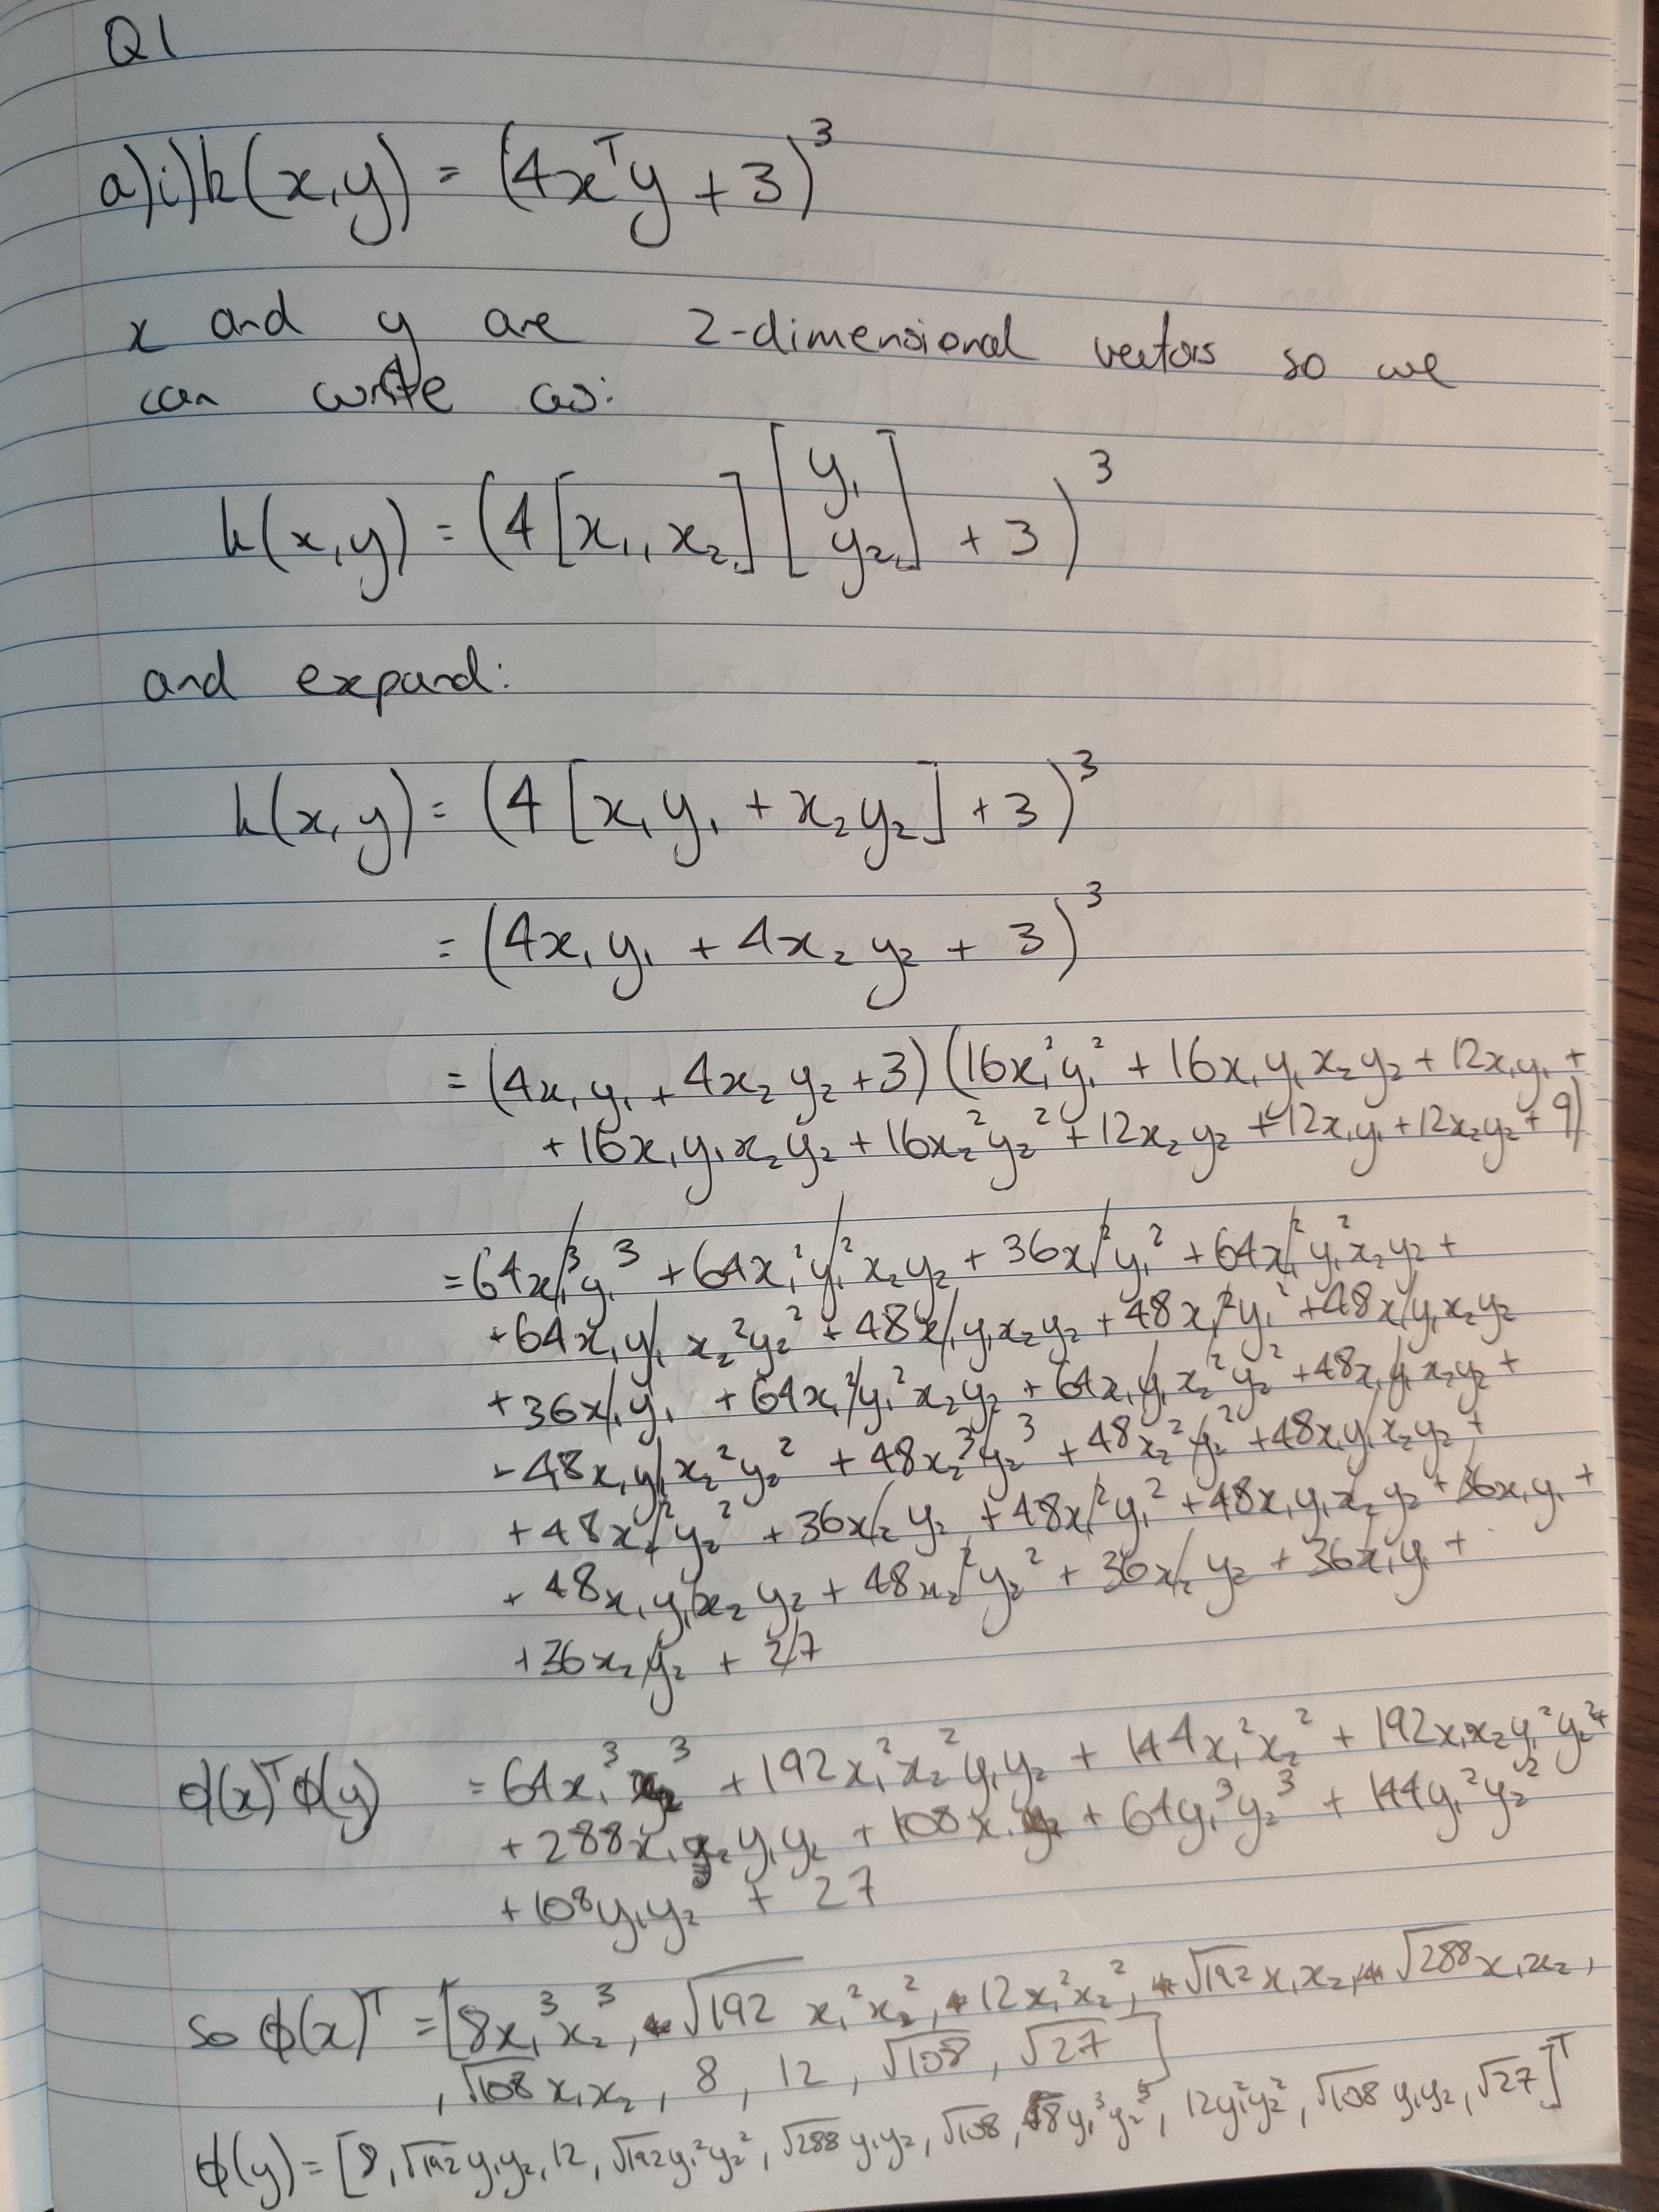
\includegraphics[scale=0.14]{q1a-i-1.jpg}
\newpage
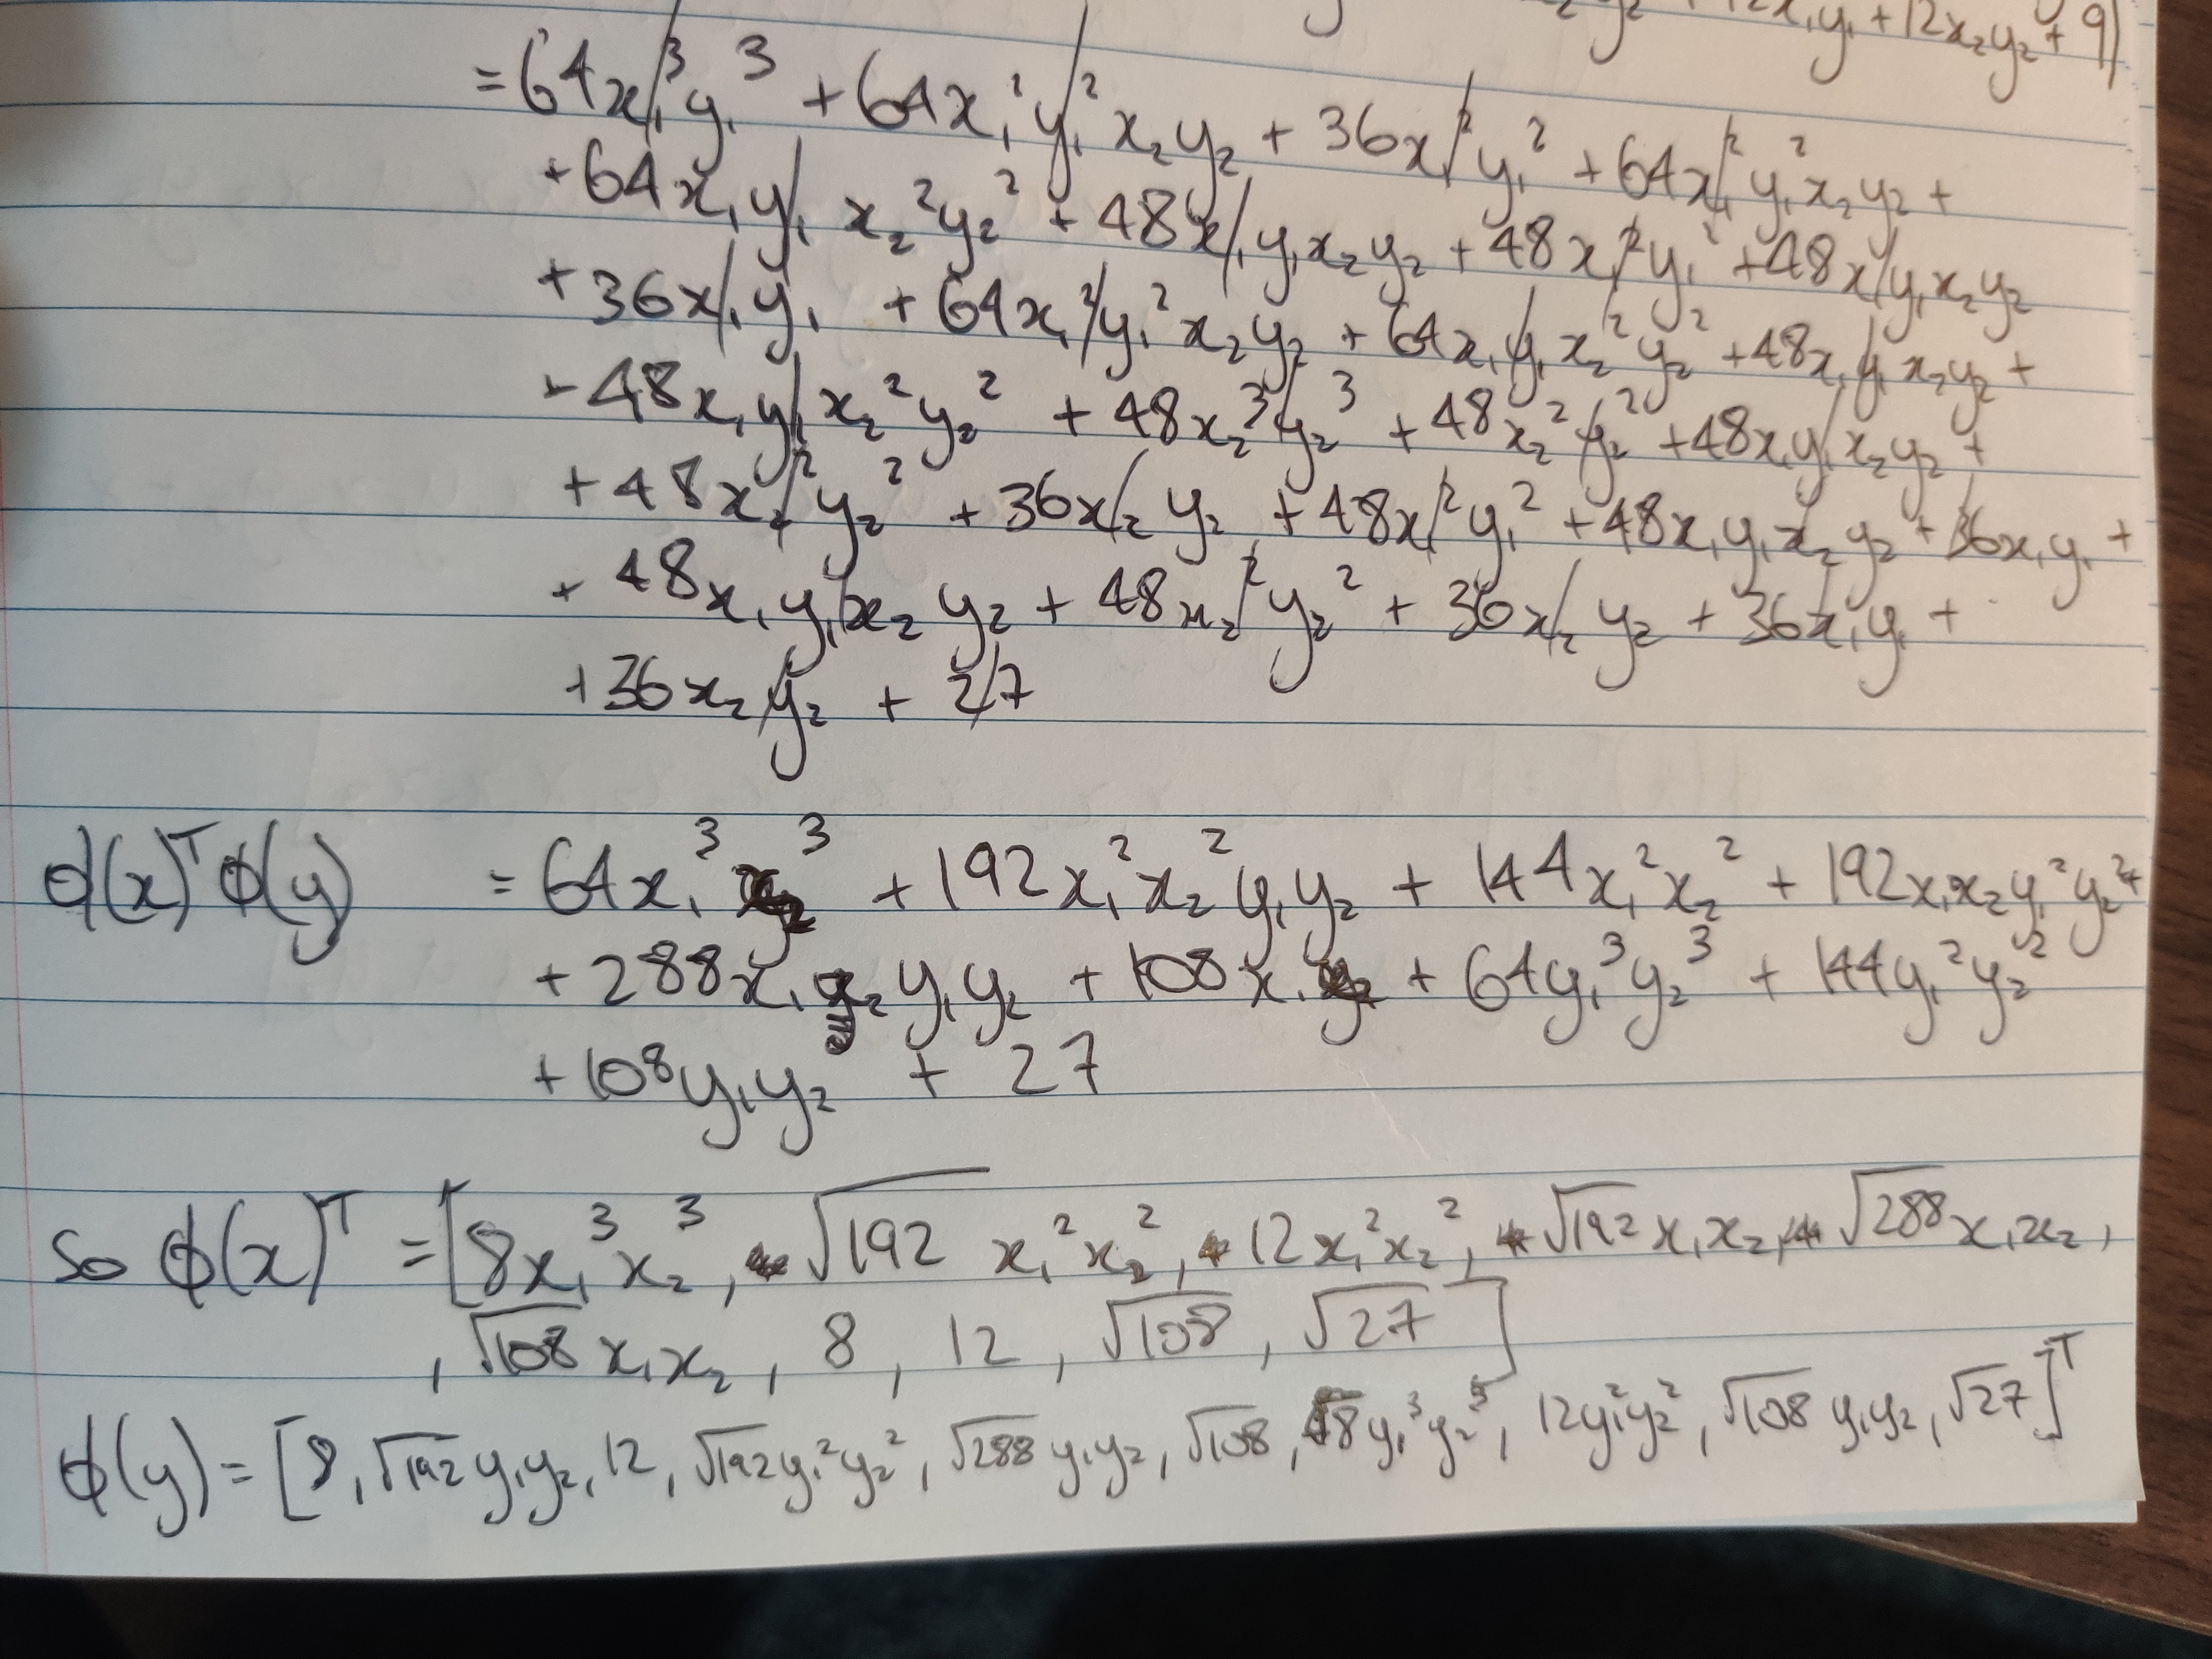
\includegraphics[scale=0.1]{q1a-i-2.jpg}

\newpage
\subsubsection*{ii}
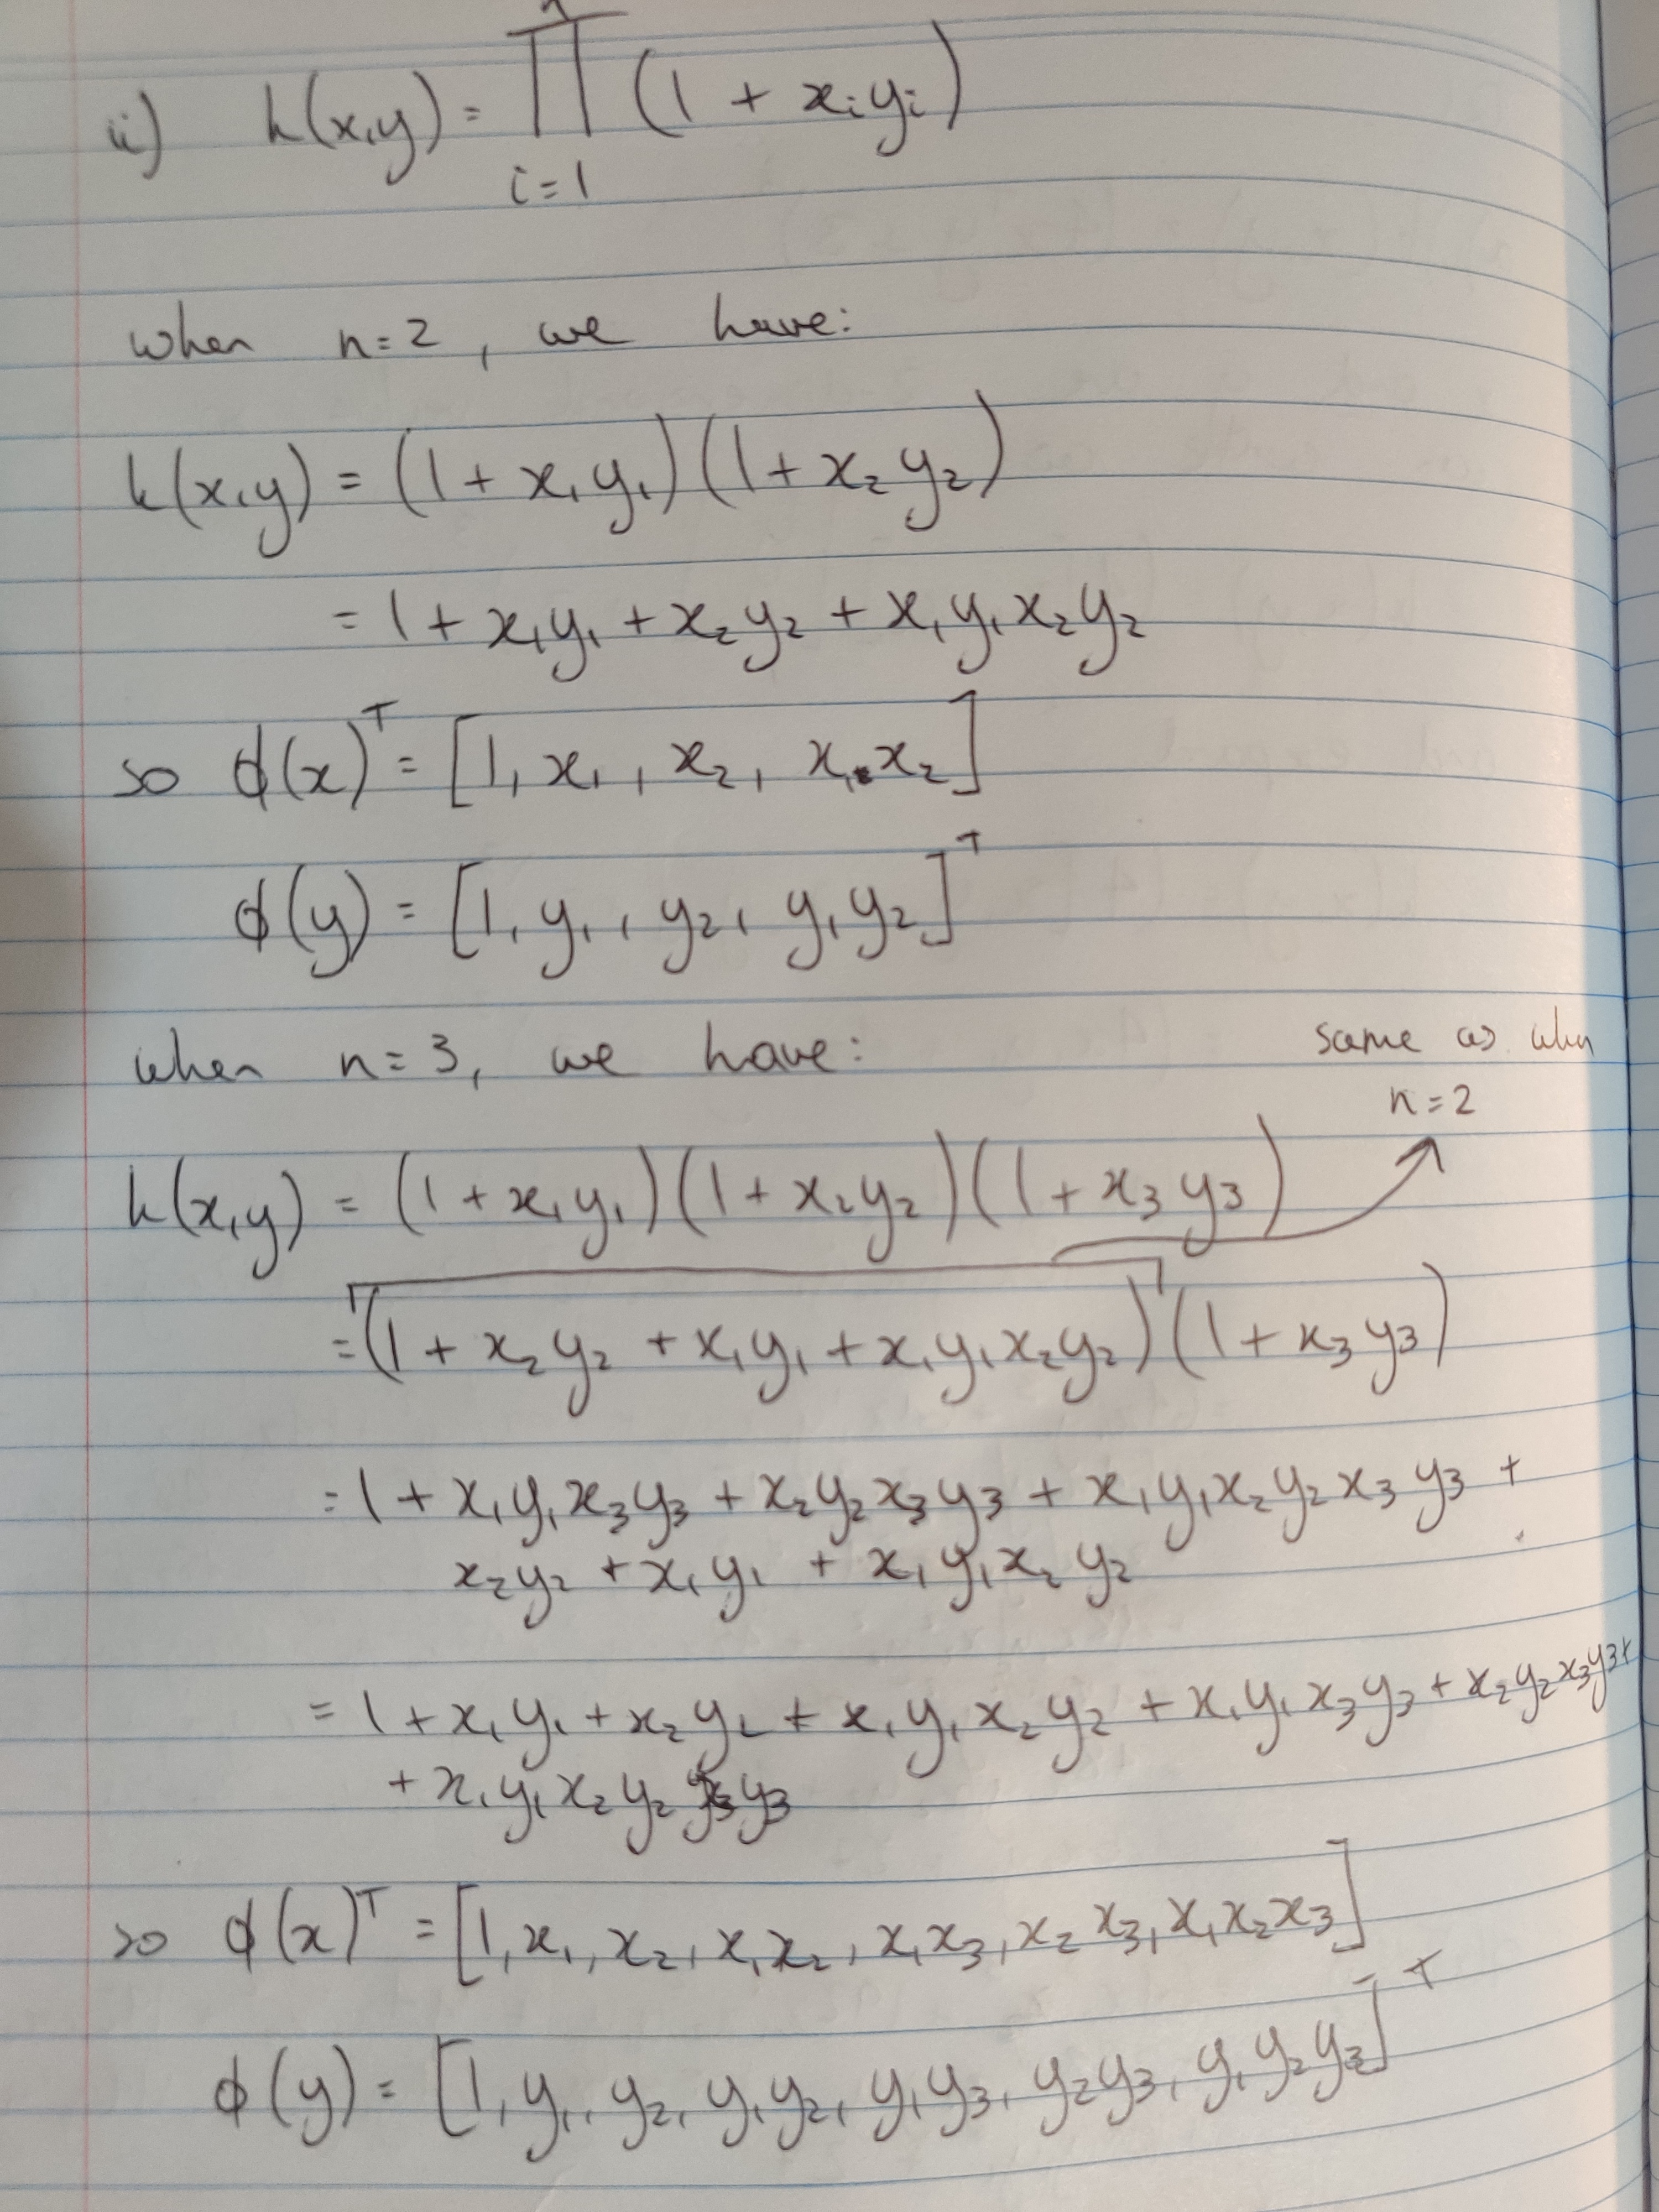
\includegraphics[scale=0.14]{q1a-ii-1.jpg}
\newpage
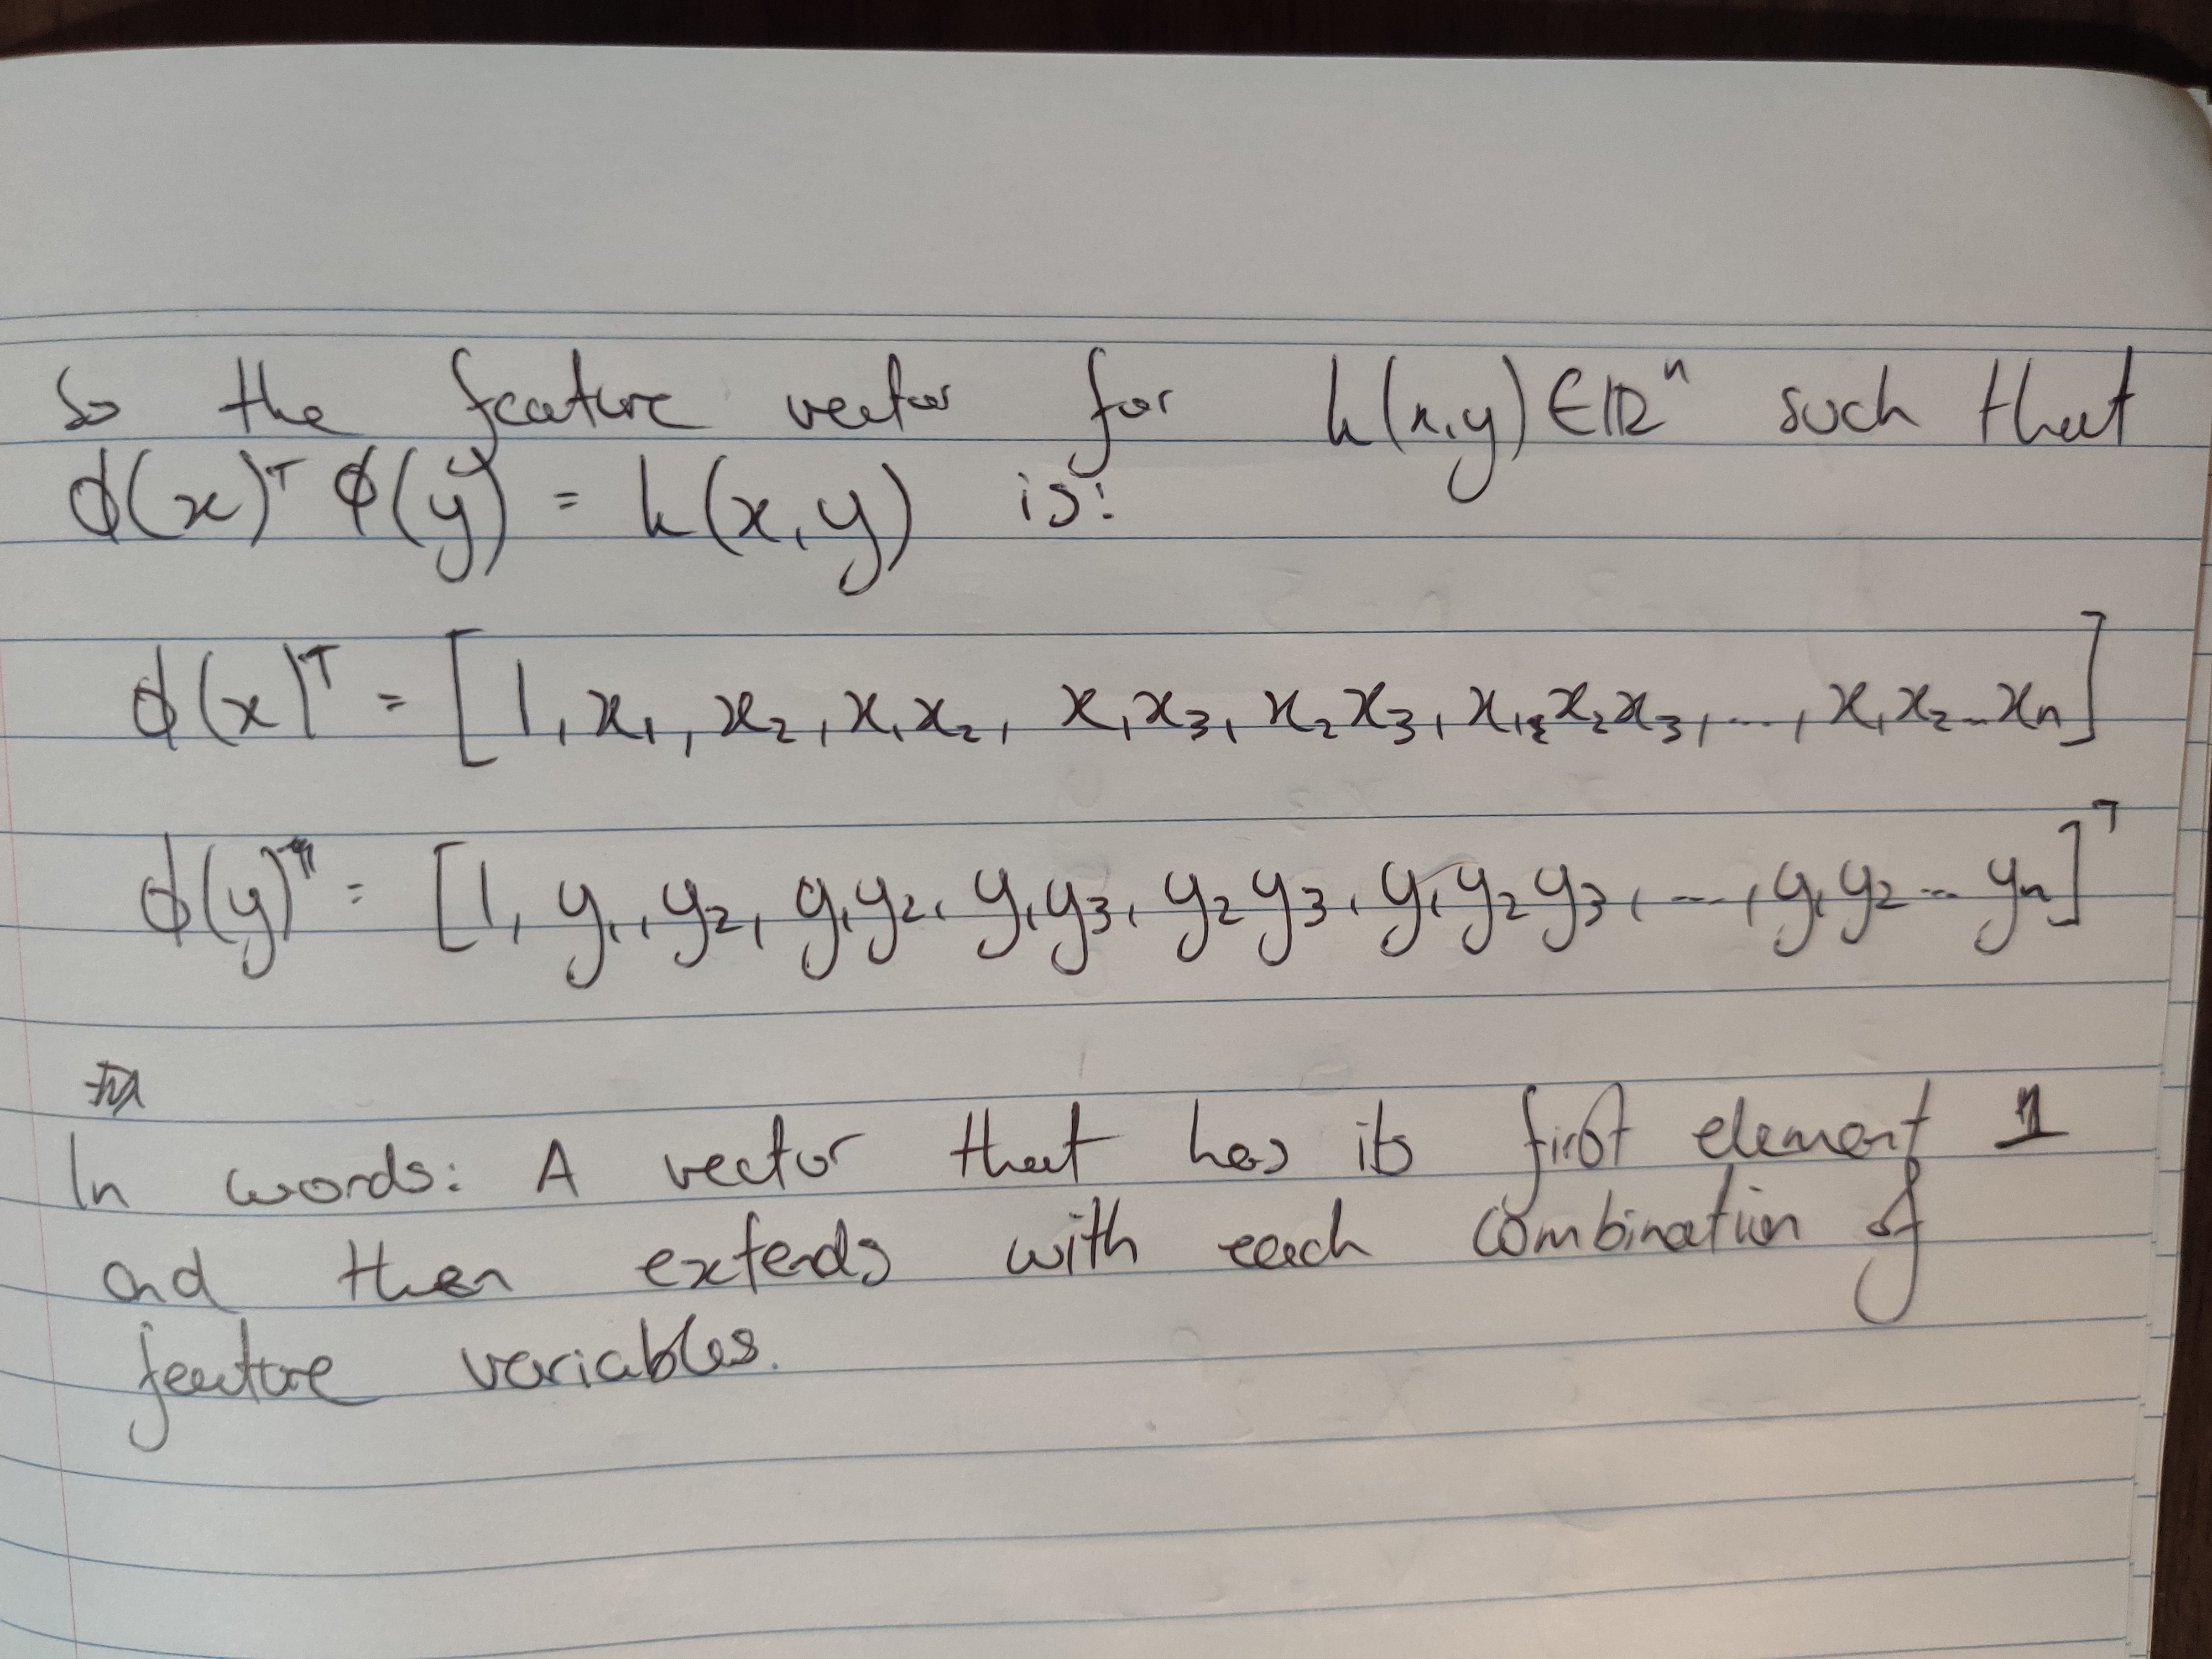
\includegraphics[scale=0.1]{q1a-ii-2.jpg}

\subsection*{b}

In these regression schemes, \(w_{0}\) acts as the y-intercept of the model and \(w_{1}\) acts as the gradient. Therefore we would expect 
regression scheme (i) to have a larger gradient than (ii) since there is a smaller penalty on \(w_{1}\) (\(\lambda = 1\) vs \(\lambda = 10\) respectively).
Regression schemes (iii) and (iv) would have a smaller y-intercept than (i) and (ii) since \(w_{0}\) is included in their penalties. Scheme (iv) would have 
a smaller gradient and y-intercept than (iii) since its penalty hyperparameter is larger (\(\lambda = 10\)).\\

From the above reasoning:
\begin{itemize}
    \item \textbf{(i) matches (a)}: (i) has the largest gradient
    \item \textbf{(ii) matches (b)}: a smaller gradient than (i) but the highest \(w_{0}\) since this is not in the regression's penalty term
    \item \textbf{(iii) matches (c)}: a relatively small gradient y-intercept
    \item \textbf{(iv) matches (d)}: (iv) has a large penalty hyperparameter so the model would be encouraged to have a small gradient and y-intercept. (d) has the smallest y-intercept and a relatively small gradient
\end{itemize}

\subsection*{c}

\subsubsection*{i}

The expected error when testing on the training data and \(k = 1\) is 0. Assuming no contradictions in the data, then because the testing data set is 
the same as the training data set and \(k = 1\), there is a classification region for each data point which will correctly classify the original training set.

\subsubsection*{ii}

There are 10,000 data points in total. 50\% of these are positive classes and 50\% are negative classes. In leave-one-out cross validation on 1NN, the data point being considered will be correctly classified if its nearest neighbour 
(but not the data point itself, since we are leaving this out) matches its classification. Even though the distribution classifications varies depending on 
the region of the dataset (e.g. the left rectangle has 25\% +ve and 75\% -ve), each rectangle has the same number of data points so if you are choosing any data point randomly in either rectangular region,
then the probability of that the data point's nearest neighbour matches its classification is 50\%. Therefore the expected error is 5,000.

\subsubsection*{iii}

% Looking at each rectangle, the left rectangle in the test data has no +ve classes whereas in the left rectangle in the training data there are 1,250 (25\%).
% Similarly for the right rectangle in the test data there are no -ve classes but the right rectangle in the the training data has 1,250 (25\%).
Training a 1NN model on the left rectangle of the training data will result in 25\% of the rectangle being a region that classifies a point as +ve class and 
75\% of the rectangle being a region that classifies a point as a -ve class. The left rectangle of the testing data is entirely -ve classes and 
since the data points in the test data are uniformly randomly, each data point has a
75\% chance of landing in a region that classifies the point as negative and therefore correctly. The same is true for the right rectangle region.
So overall, a 1NN model trained on the entire training dataset is expected to correctly classify 75\% of the test data giving it an expected error 
of 2,500.

\subsubsection*{iv}

Looking at the left rectangle of the training data and using 21-NN, you would expect the model to classify the entire region as -ve classes. 
This is because for each point in the left rectangle, of the 21 nearest neighbours, you would expect 25\% to be +ve and 75\% to be -ve so
overall the region is classified as negative. When the training data is used as test data, we know that the 1,250 points that are +ve will 
be incorrectly classified as -ve and therefore the expected error is 1,250. This is the same for the right rectangle however the classifications
are inverted. Overall, you would expect a training set error of 2,500 using a 21-NN classifier model.

\subsection*{d}

\subsubsection*{i}
The space of \(X\) is \(2^{p}\). The space of \(Y\) is 2. Therefore the size of the hypothesis class is \(2^{2^{p}}\).

\subsubsection*{ii}

The probability that the version space is not \(\epsilon-exhausted\) after \(n\) training examples is at most \(|H|e^{-\epsilon n}\).
The number of samples needed to ensure that the sample space has a 0.9 probability (\(P\)) of being \(\epsilon-exhausted\) is:

\[
    n = \frac{1}{\epsilon}(ln|H| + ln(\frac{1}{P}))
\]

Substitute in the values to yield:

\[
    n = \frac{1}{0.1}(ln(2^{2^{10}}) + ln(\frac{1}{0.9}))
\]
\[
    n = 10*(1024*ln(2) + ln(\frac{10}{9}))
\]
\[
    n = 7,098.88
\]

Therefore at least 7,099 data points are needed to ensure the version space is \(\epsilon-exhausted\) with 0.9 probability.

\subsection*{f}

\subsubsection*{i}
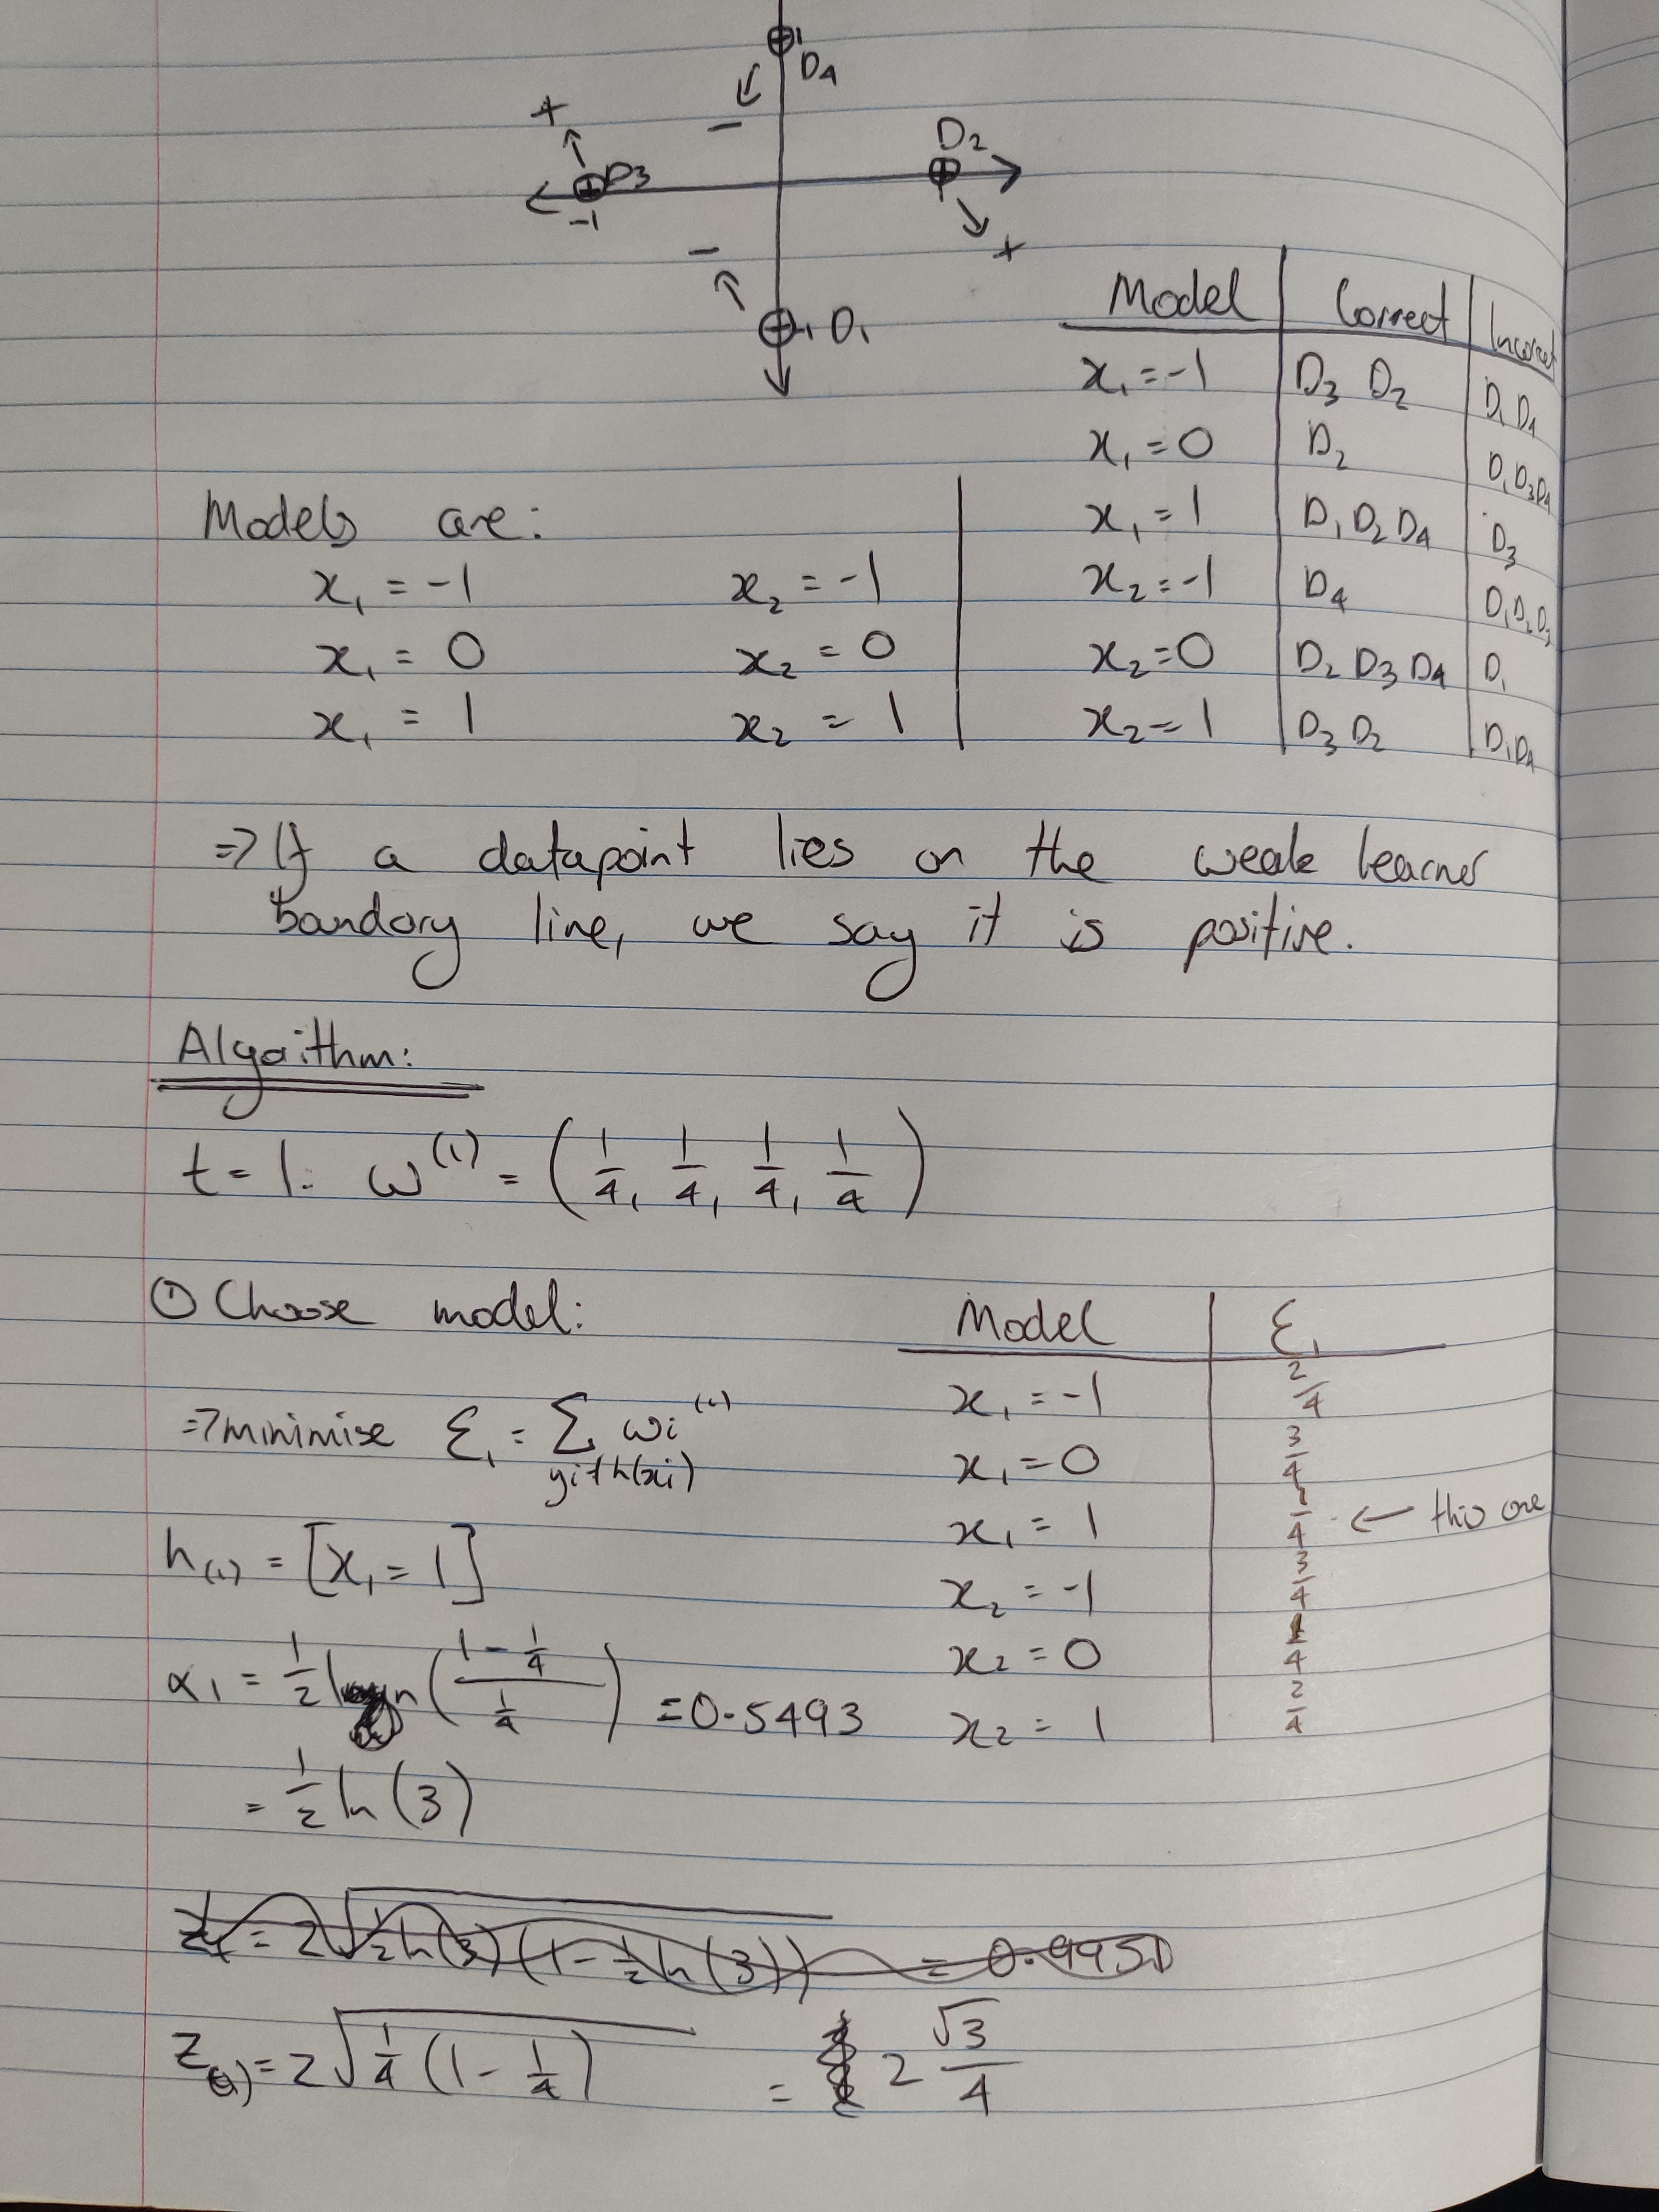
\includegraphics[scale=0.14]{q1f-i-1.jpg}
\newpage
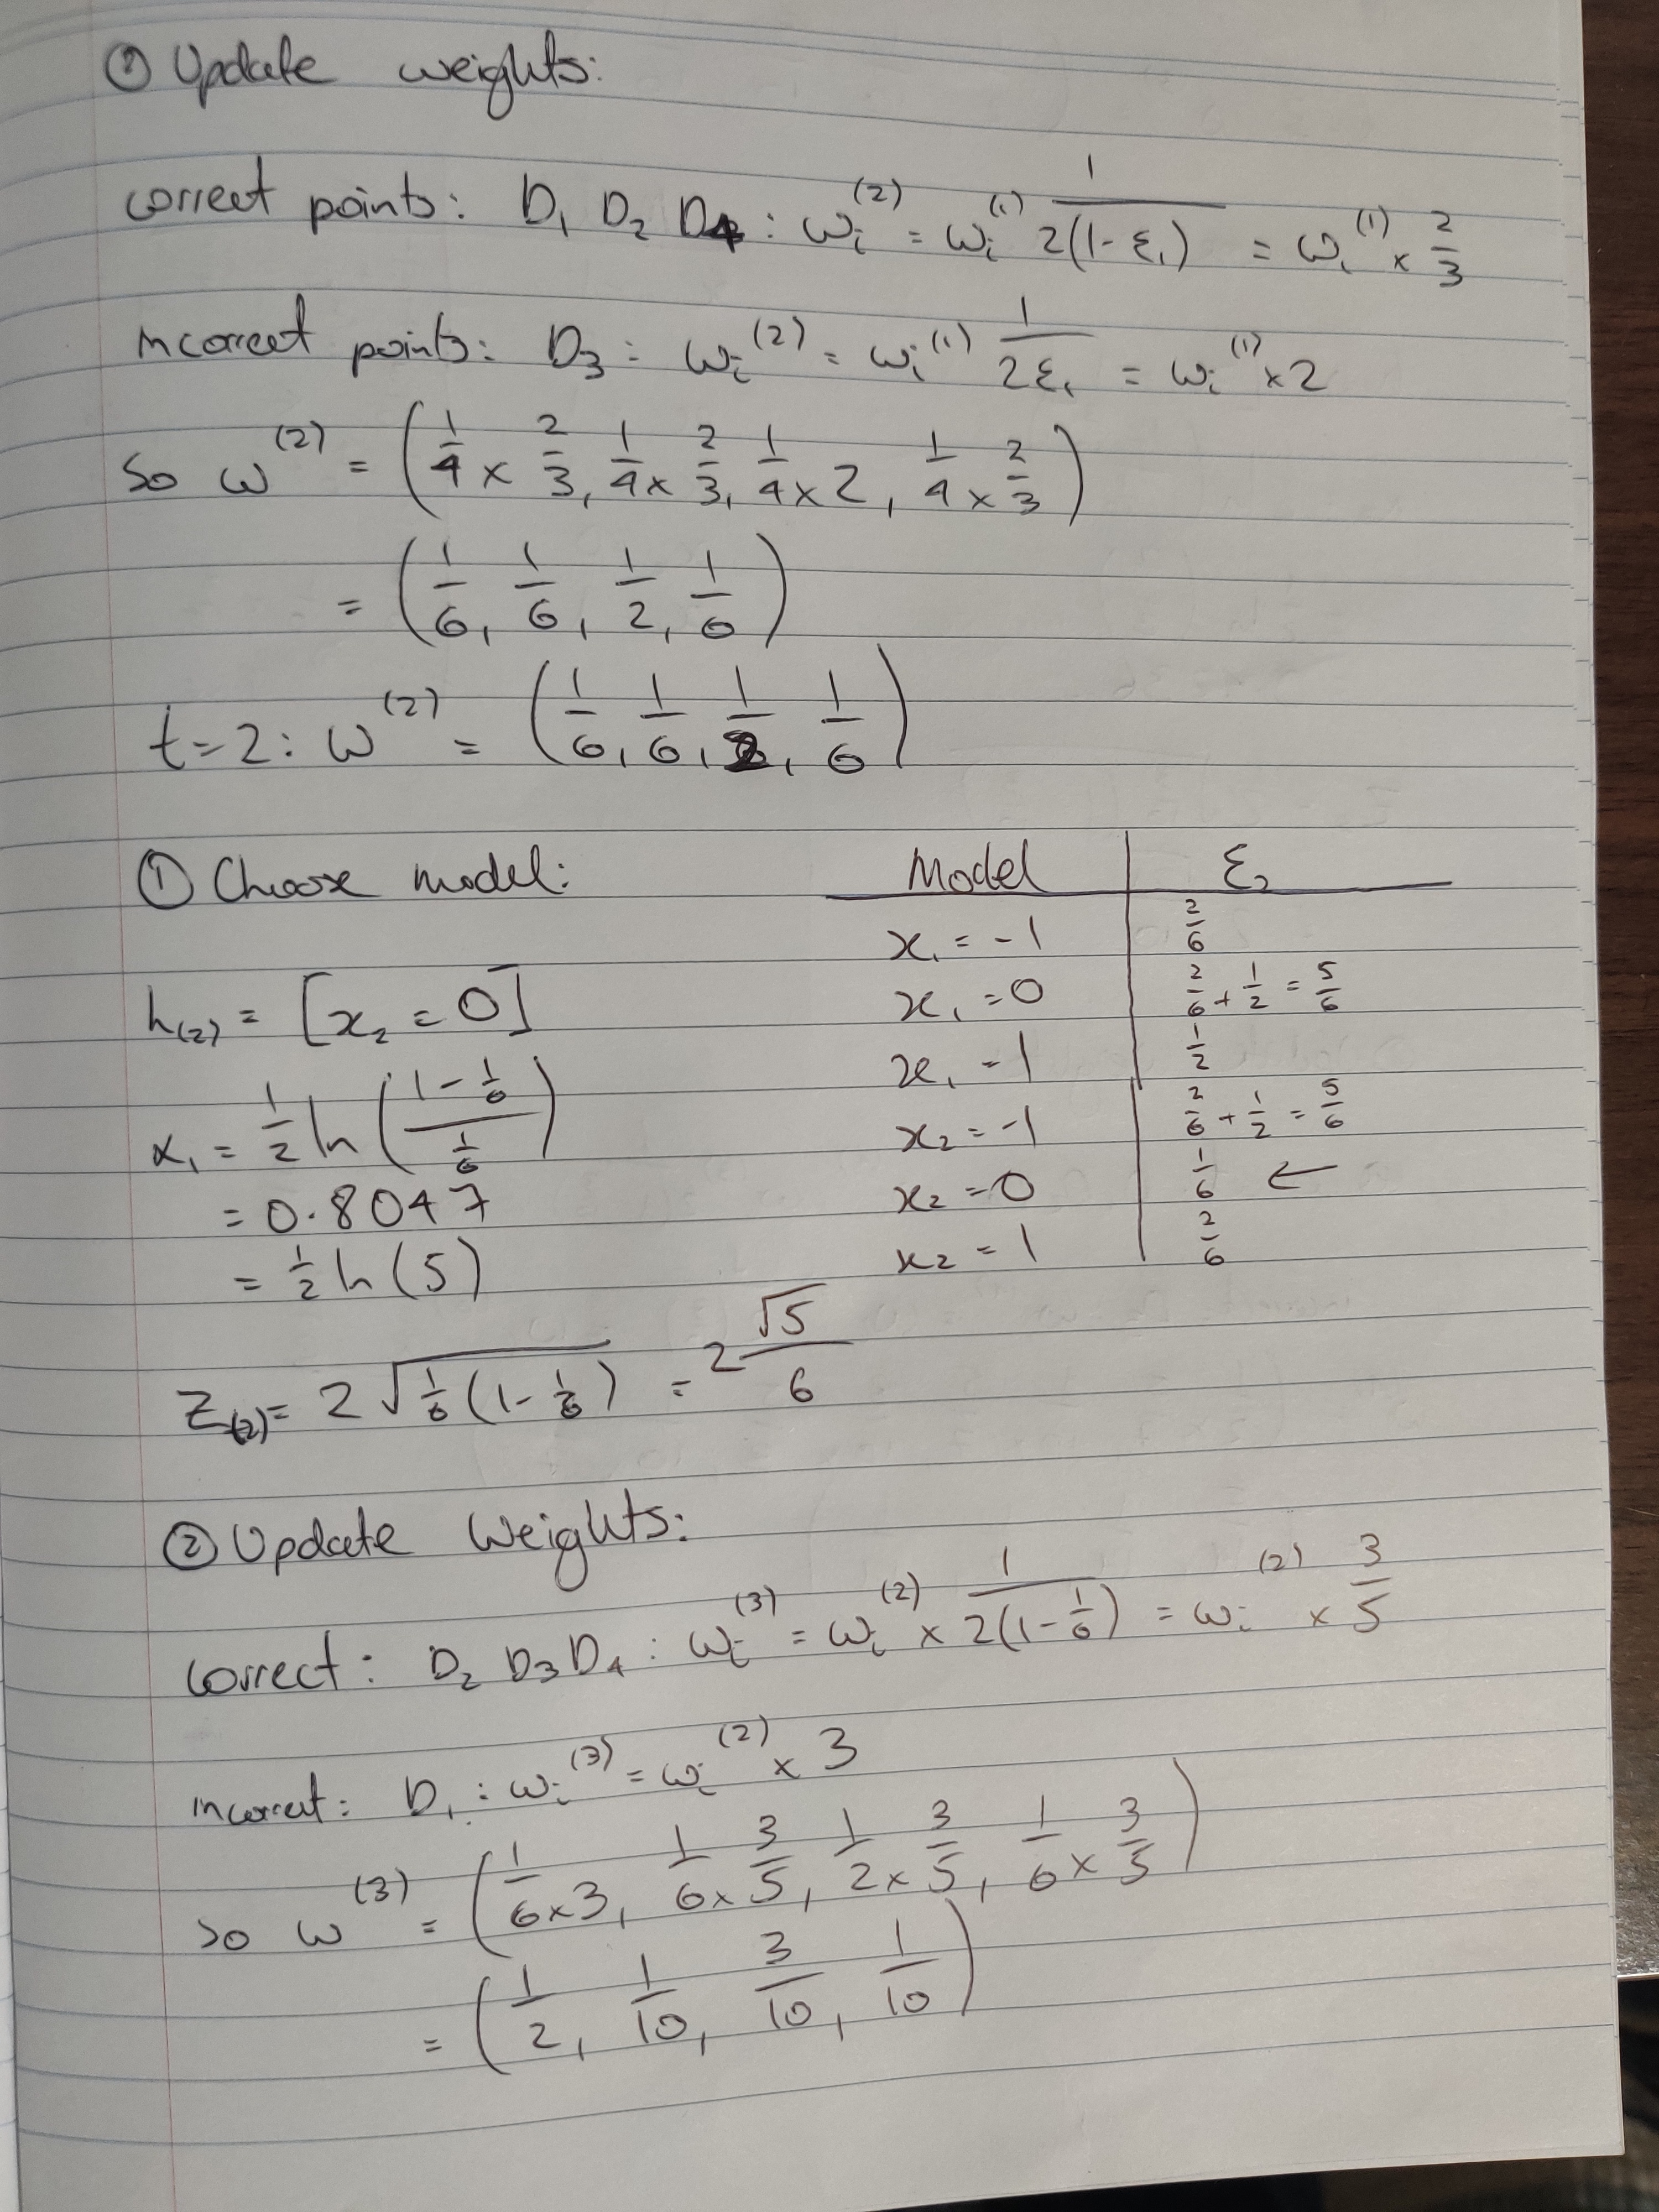
\includegraphics[scale=0.14]{q1f-i-2.jpg}
\newpage
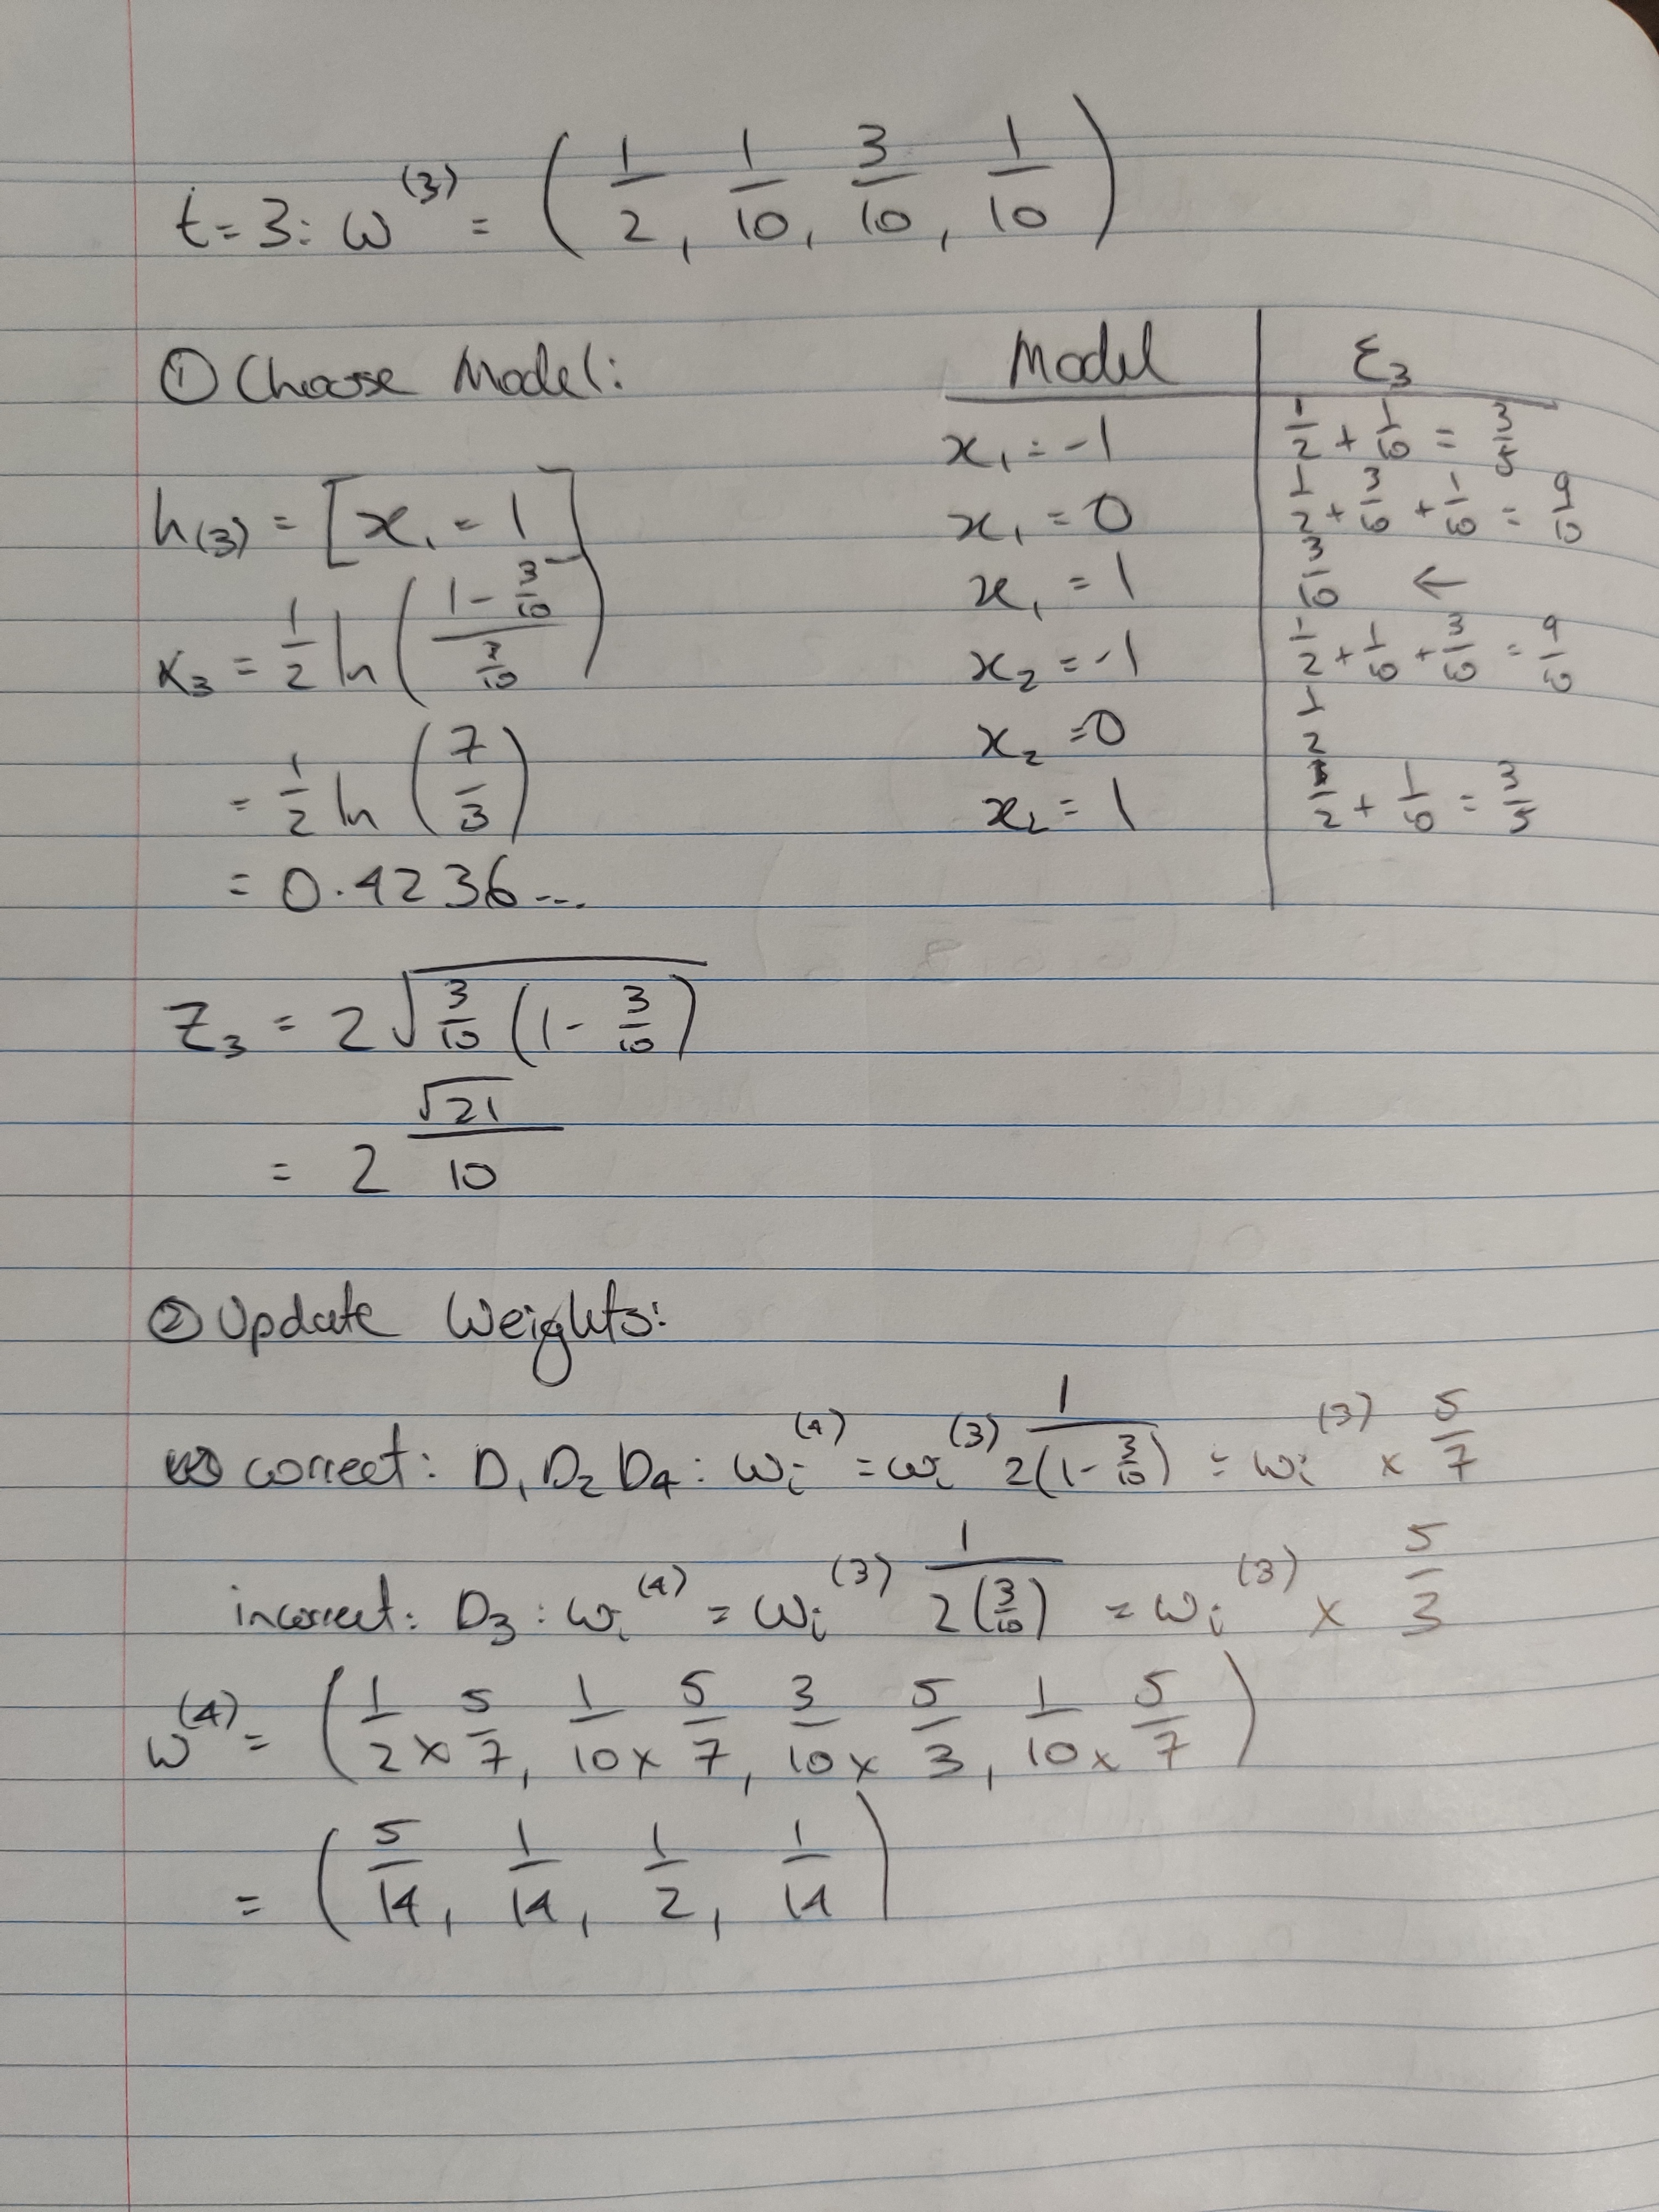
\includegraphics[scale=0.14]{q1f-i-3.jpg}
\newpage
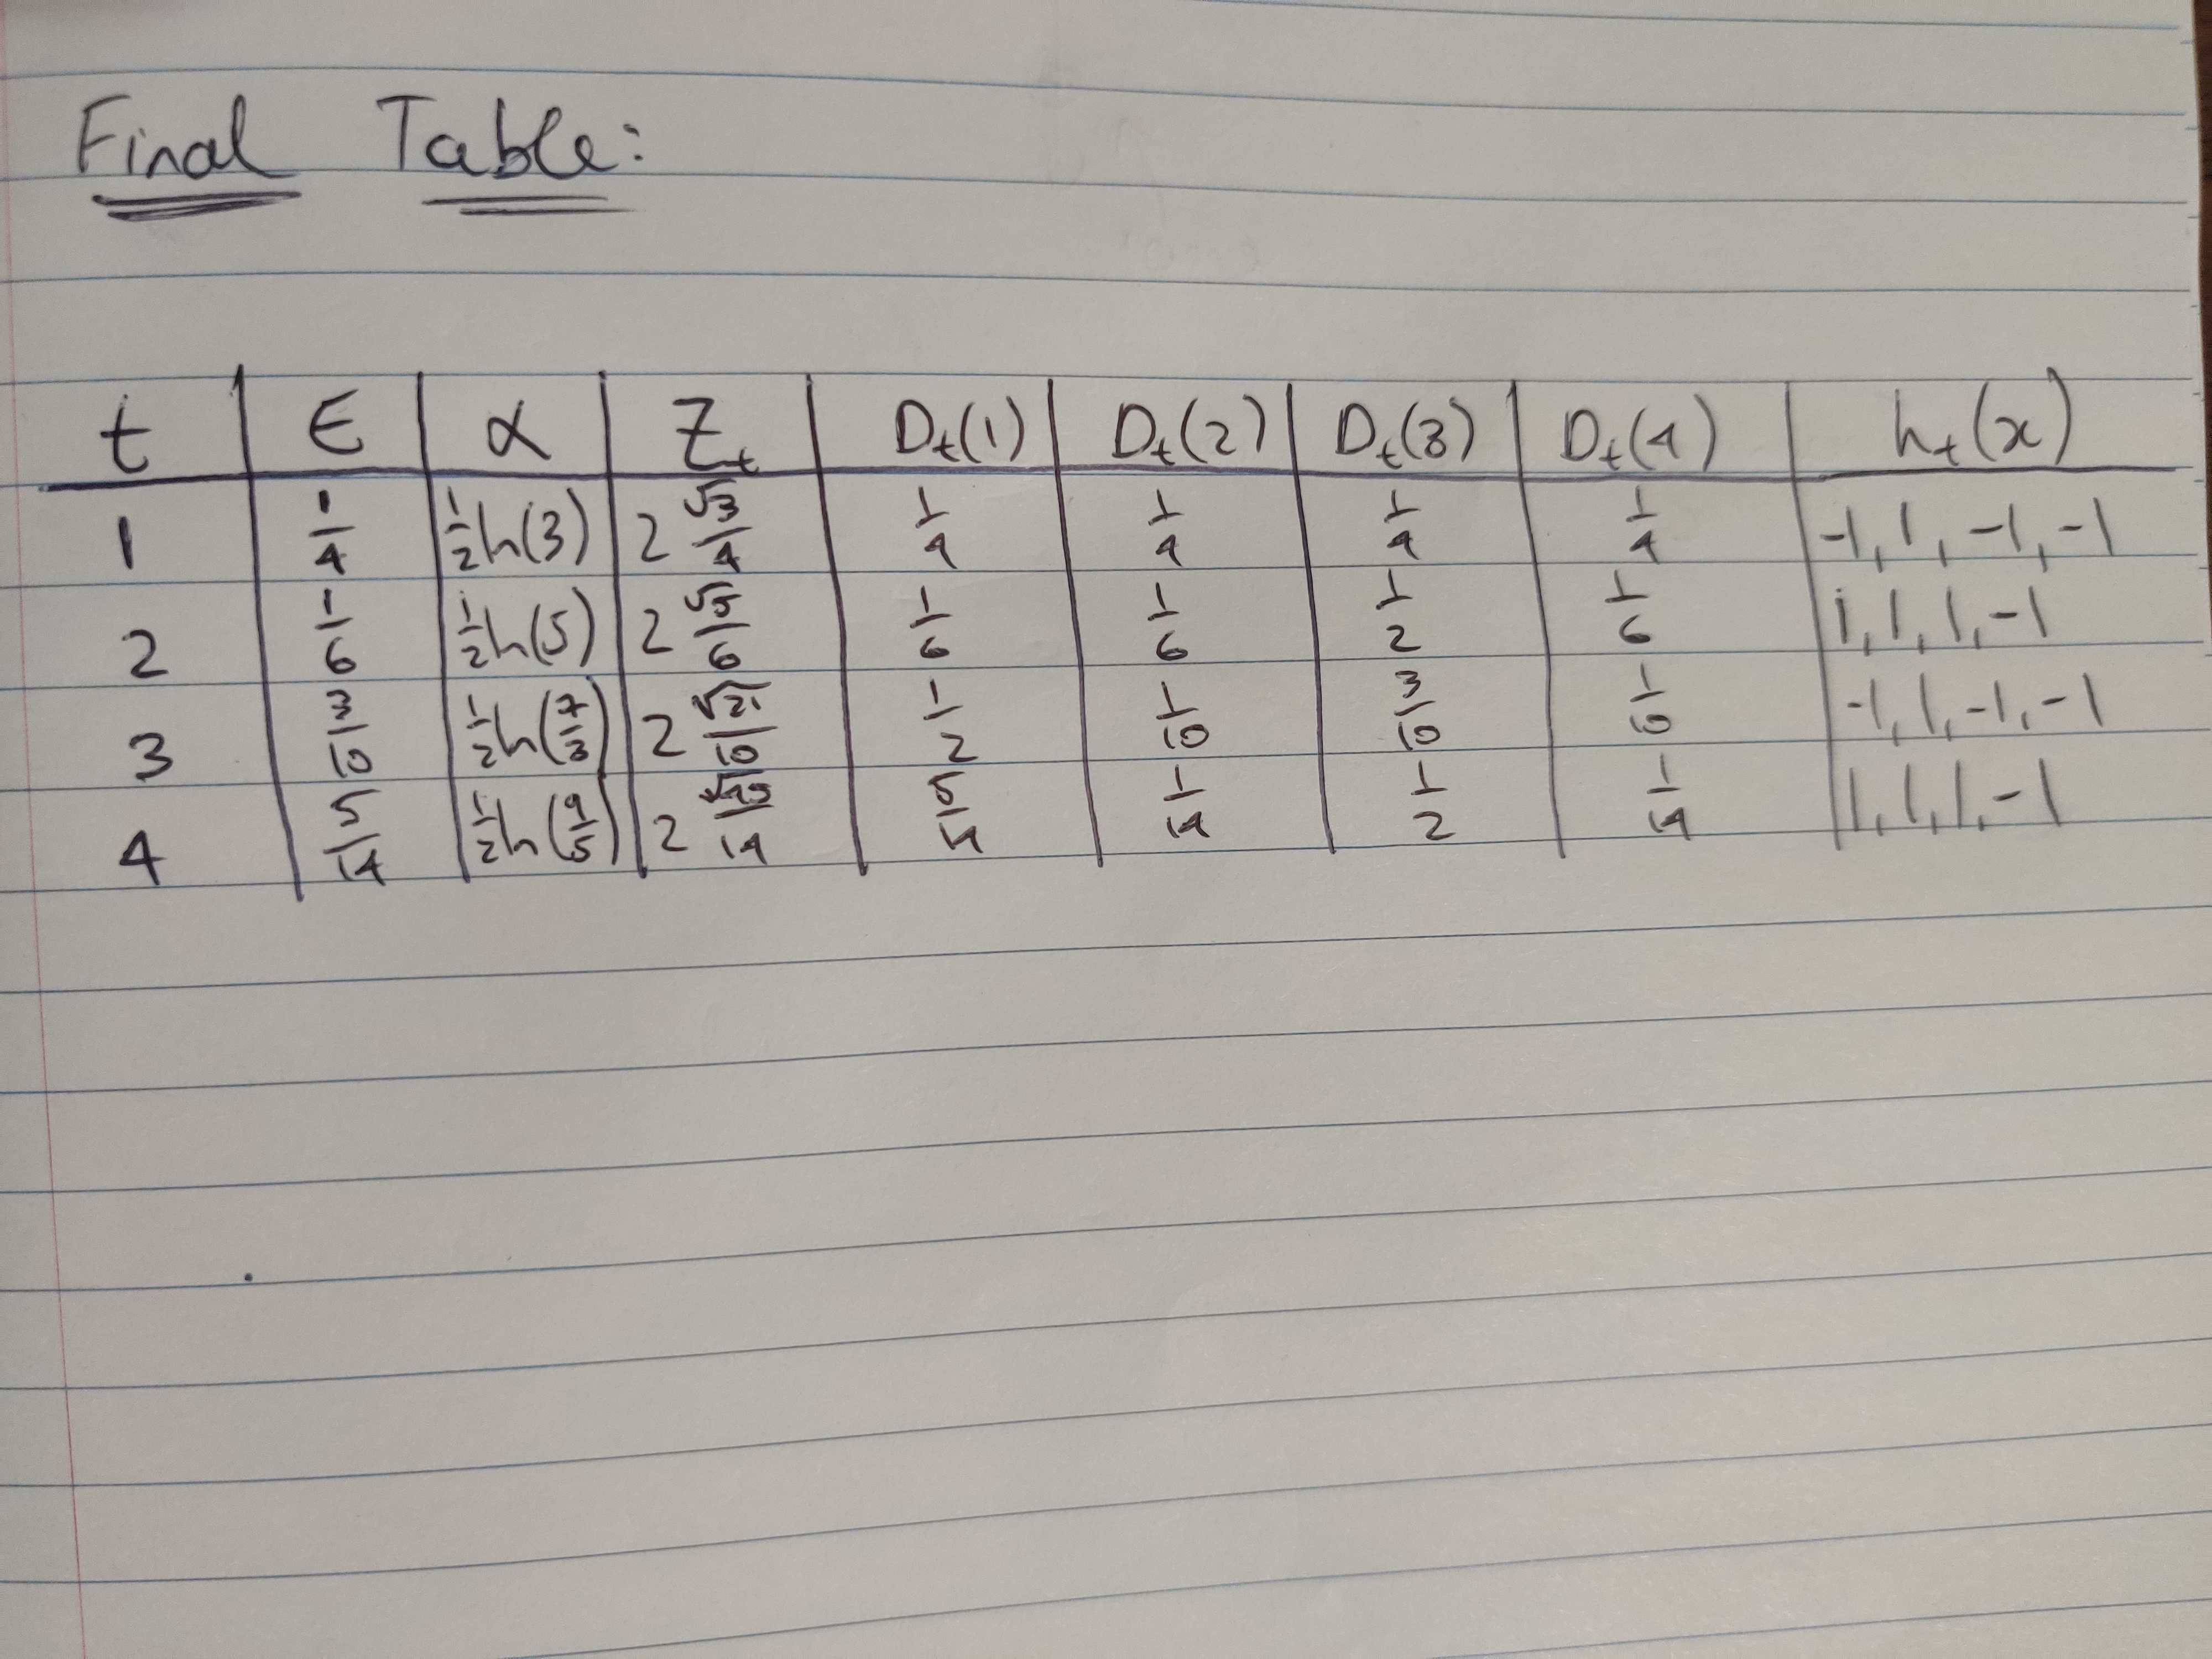
\includegraphics[scale=0.1]{q1f-i-4.jpg}

\subsubsection*{ii}
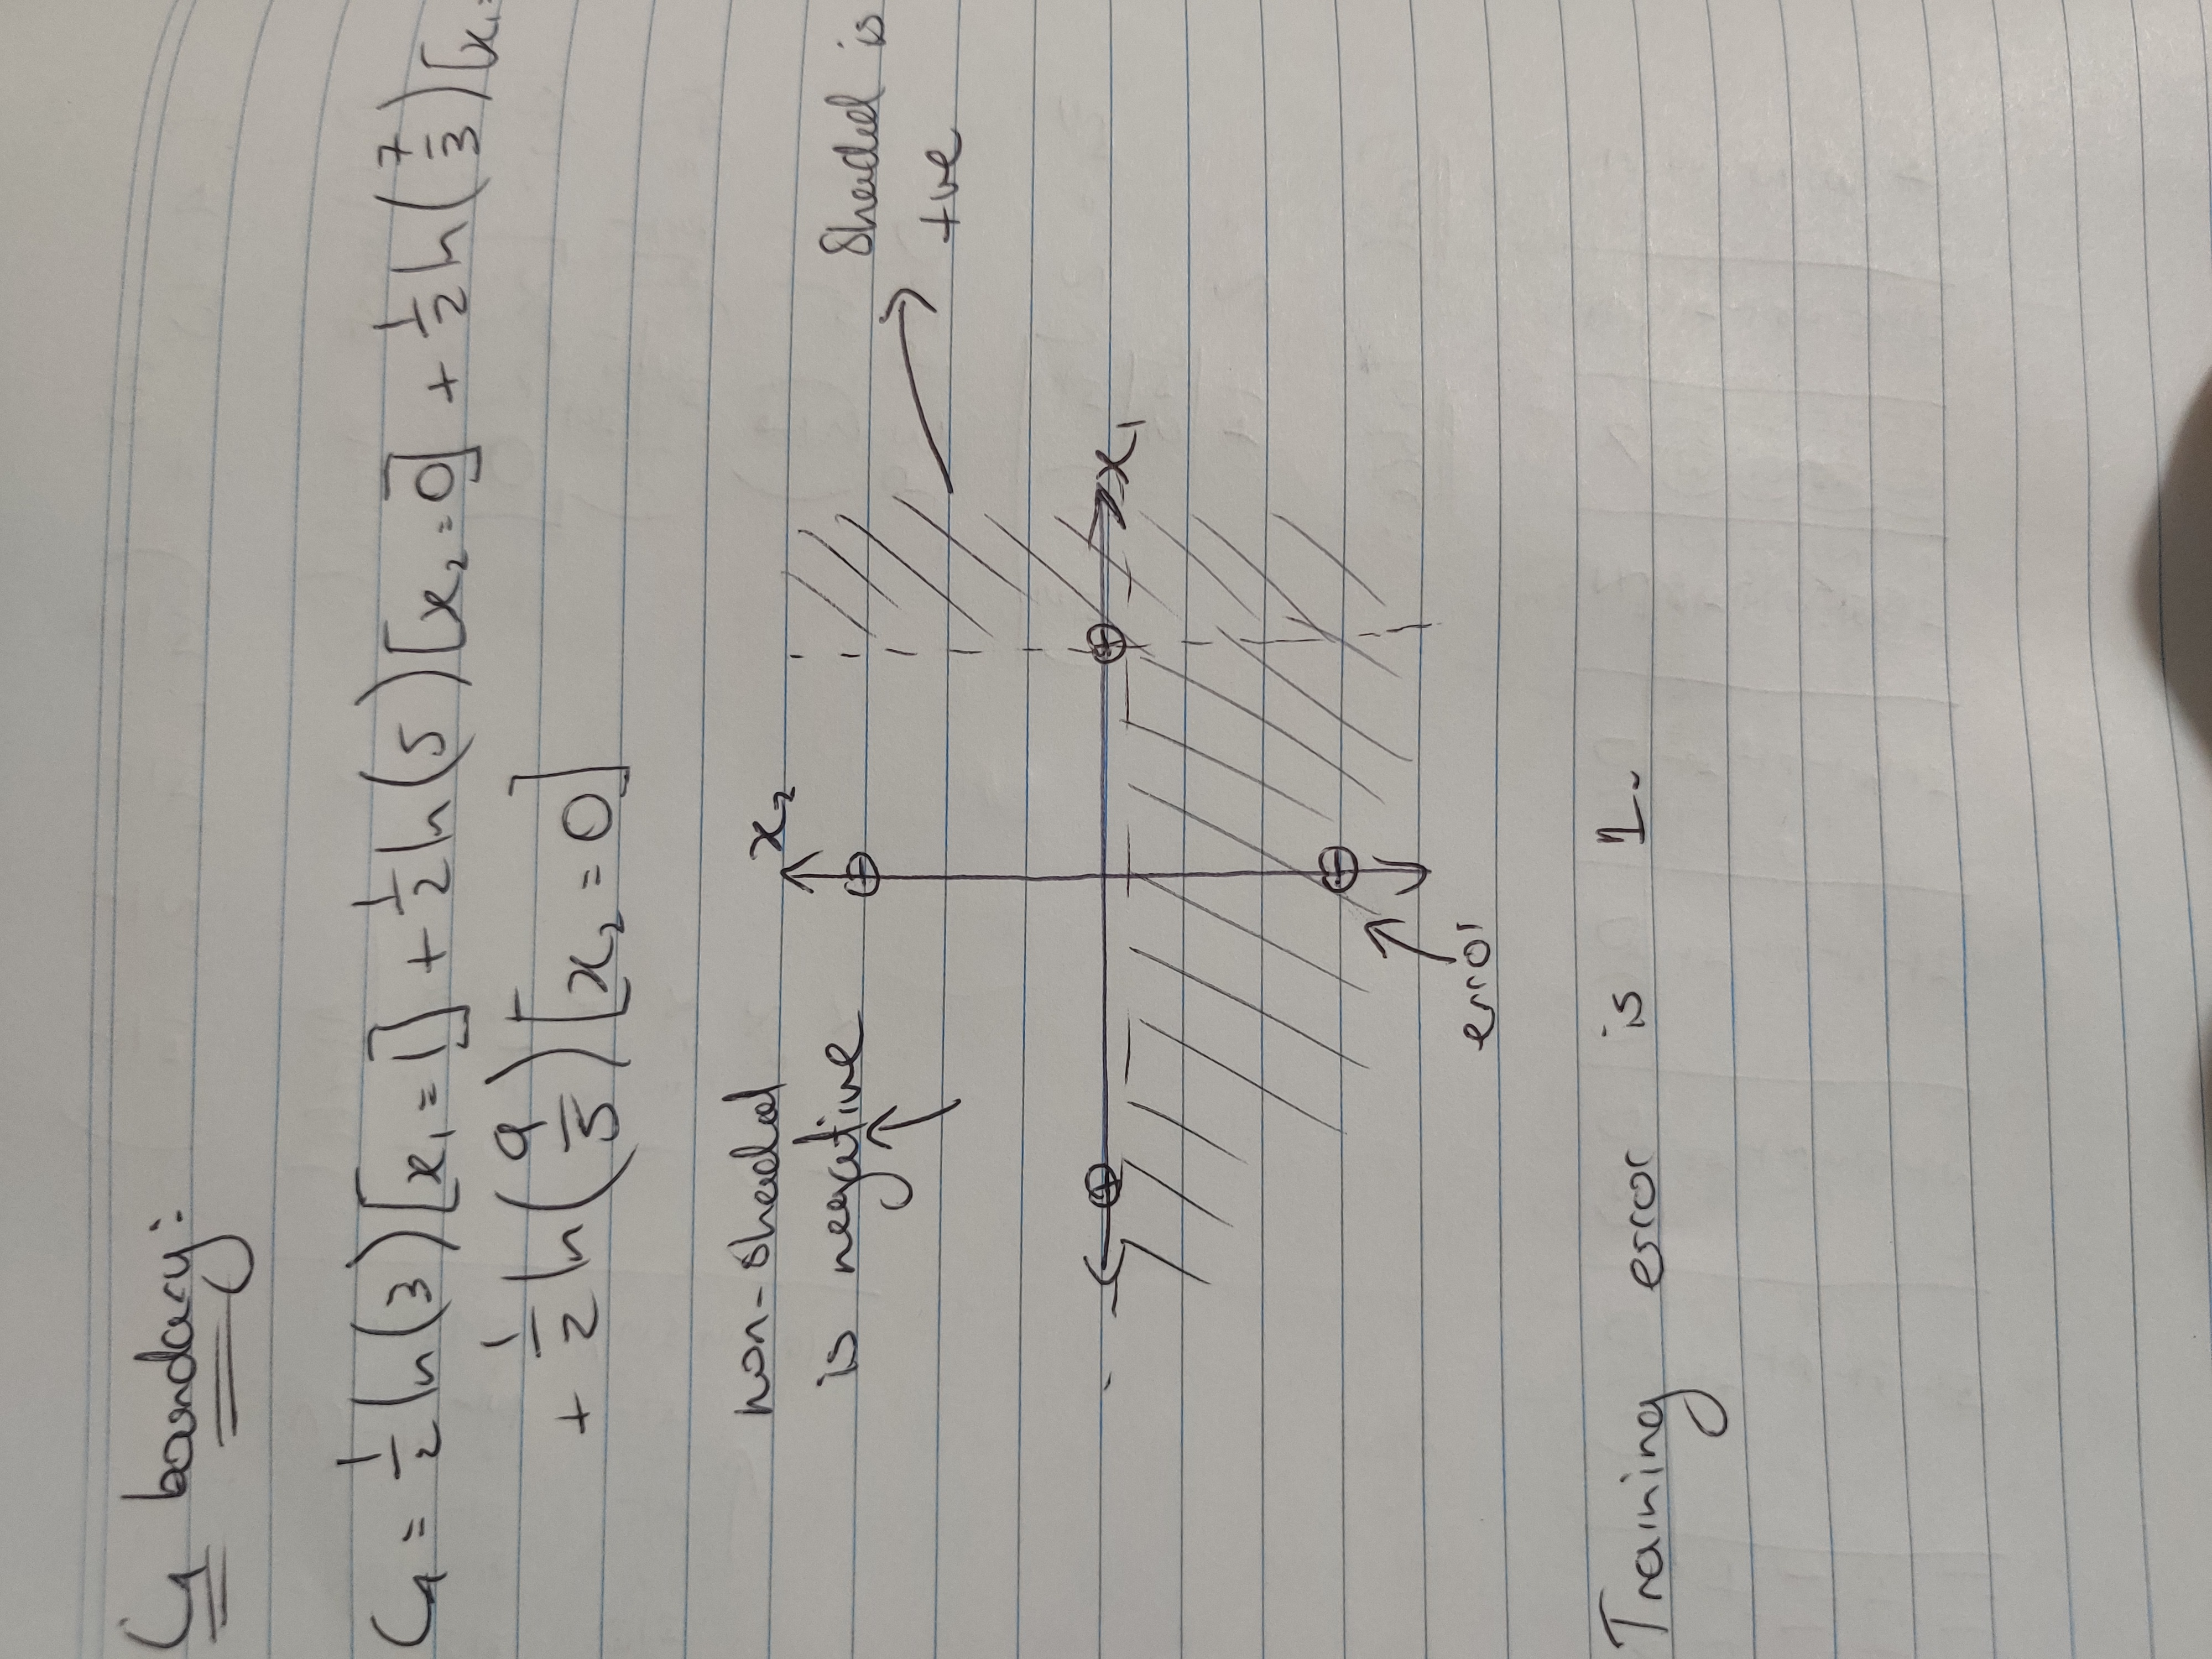
\includegraphics[scale=0.1]{q1f-ii-1.jpg}

\newpage
\section*{Question 2}

\subsection*{a}
\subsection*{i}
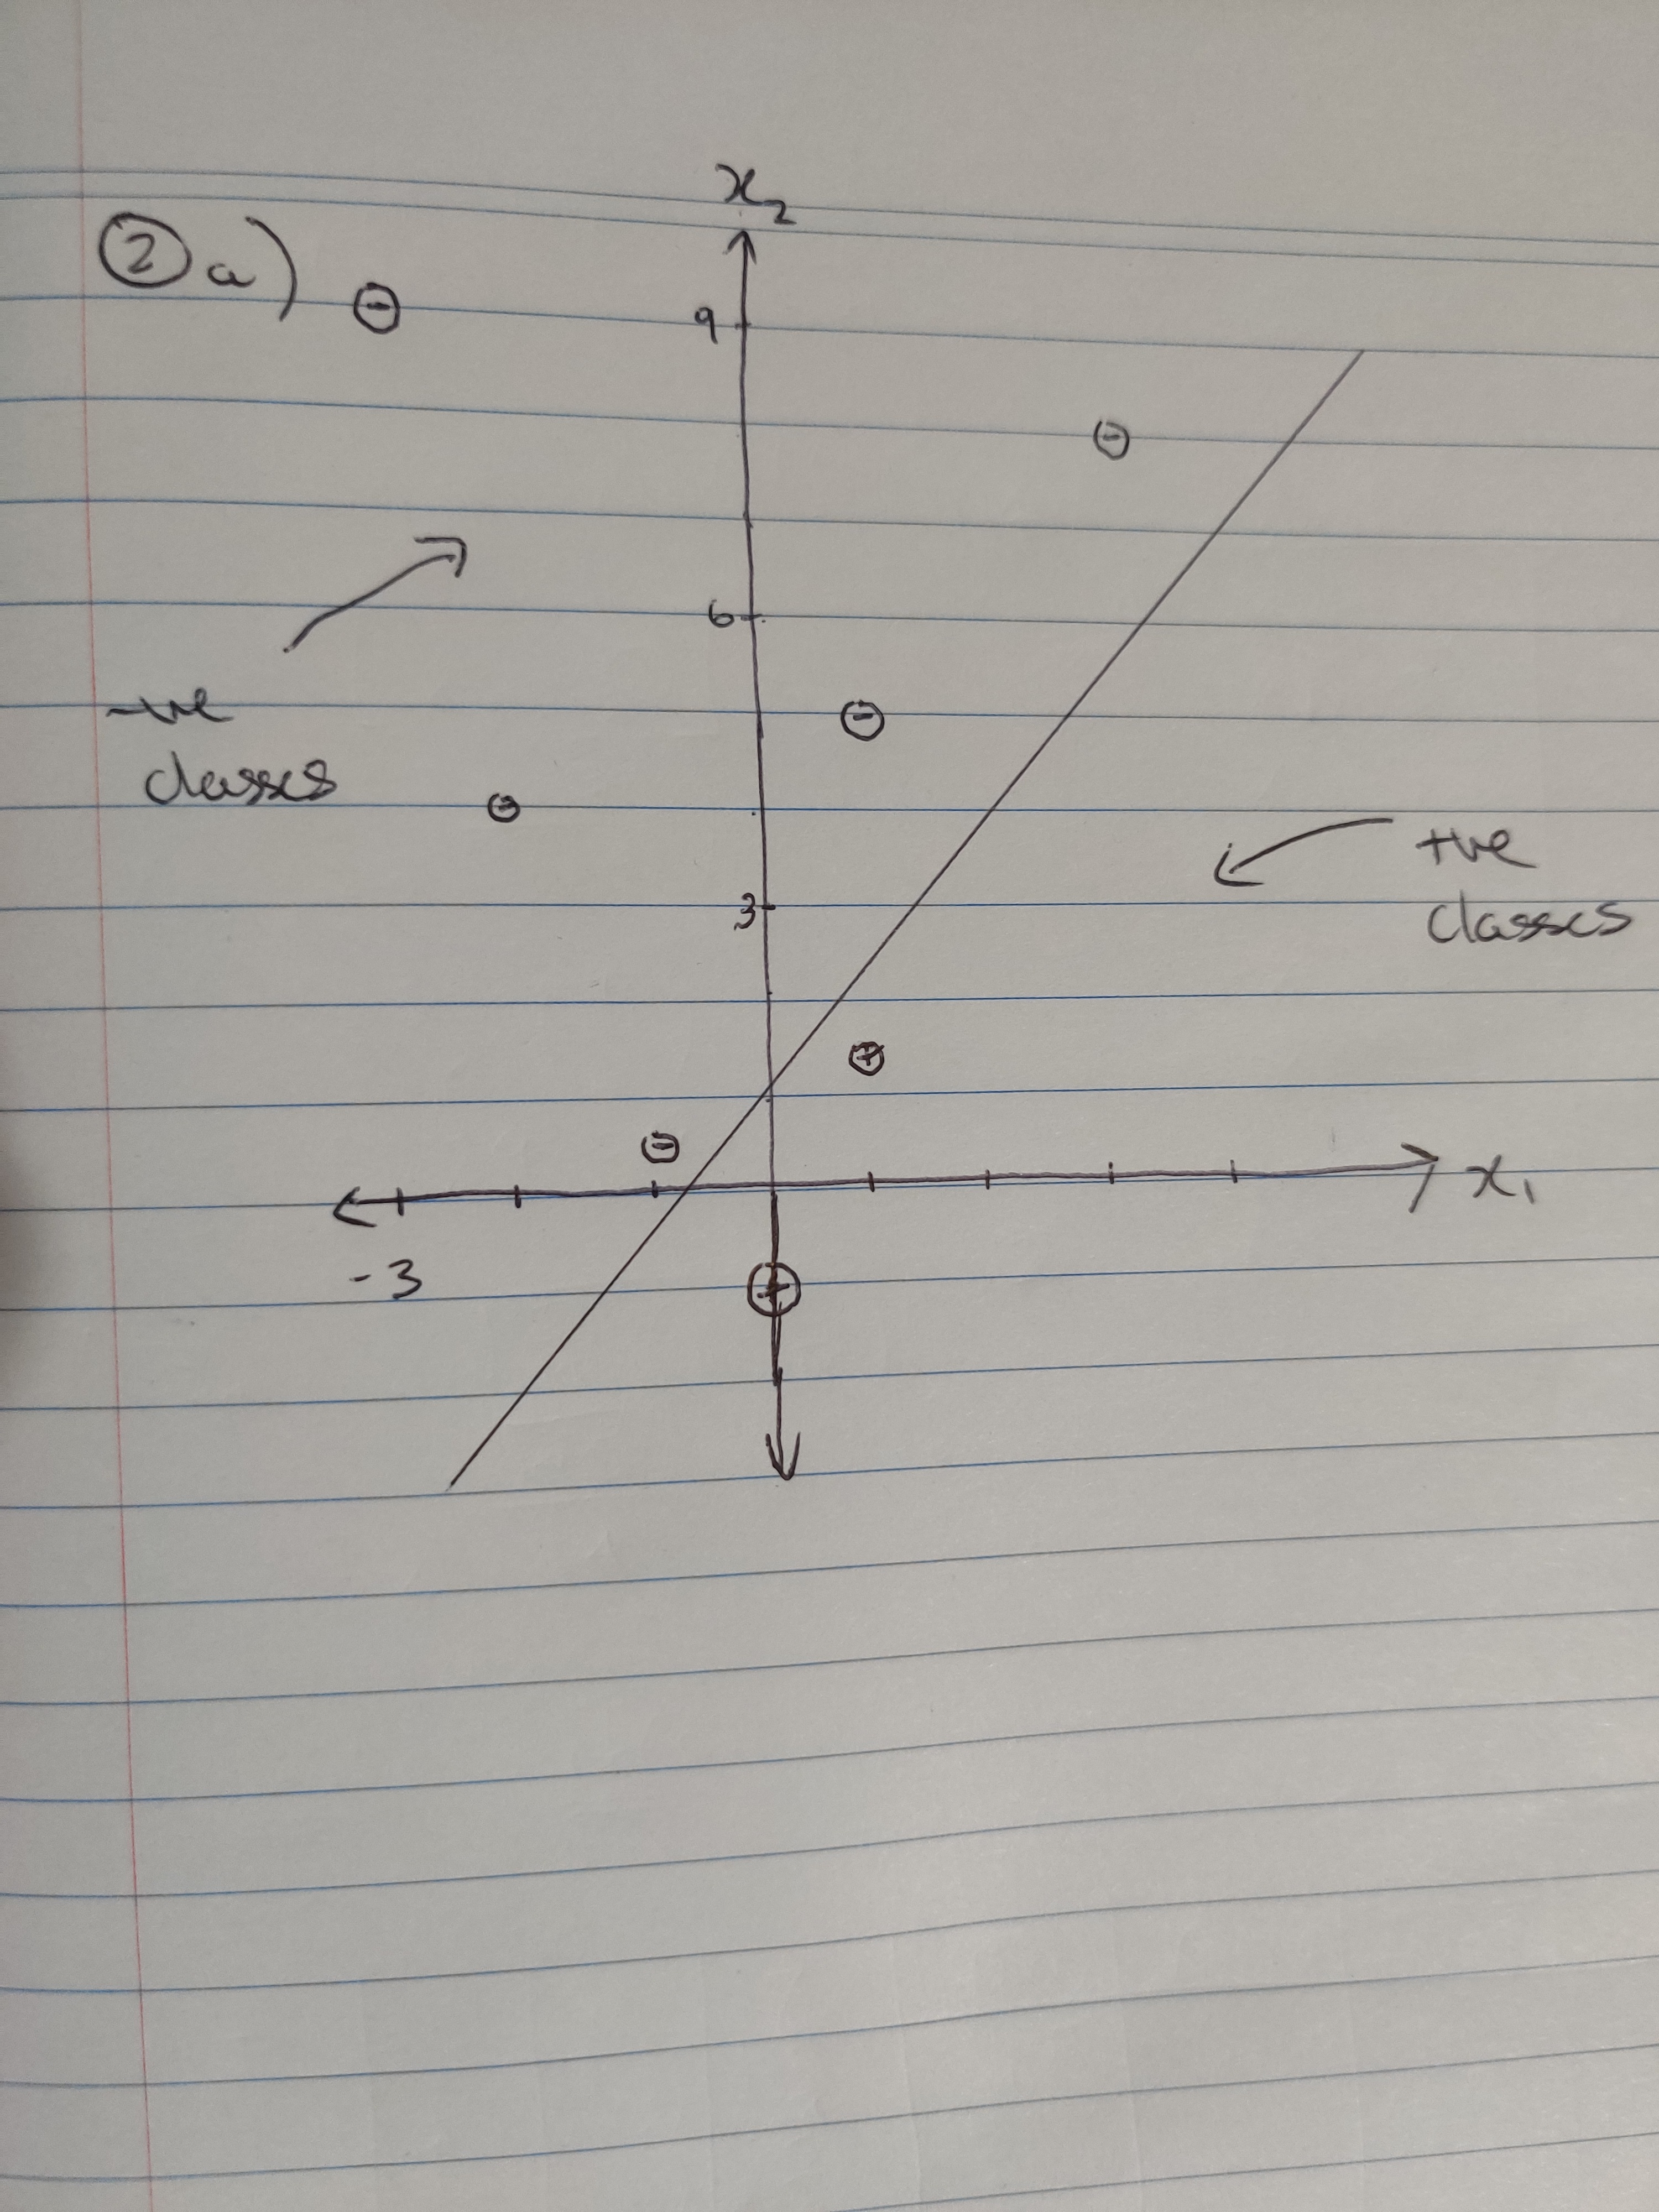
\includegraphics[scale=0.14]{q2a-i-1.jpg}

\subsection*{d}

The statement is falsifiable since SVMs do have a way to handle non-linearly separable data.
The first way is by creating a "soft margin" to accommodate for some errors. The second is by projecting
the dataset into higher dimensions such that it is linearly separable. Although the projection to 
a higher dimension comes at a computational cost, it does not affect the performance of the 
SVM. This is how SVMs can handle non-linearly separable data and why the statement 
is incorrect.

\subsection*{e}

As mentioned in (d), non-linearly separable data can be projected into higher dimensions such that it is 
linearly separable. Working in these higher dimensional spaces can come at a 
computational cost that is sometimes impractical. The \textbf{kernel trick} is a method of dealing
with this problem by representing the data as a mapping from an input vector 
to the dot product of the vectors in the higher dimensional space. The "trick" is that this method doesn't explicitly apply the 
expensive transformation into a higher dimensional space. This is how impractical projections into higher
dimensional space can become practical, which is important for SVM and other ML methods that 
require linearly separable data and is why the kernel trick is such an important technique in machine learning.

\subsection*{f}

After the forgotten data point is added back in, the dataset it still 
linearly separable. Support vectors are instances that are closest to the
maximum margin hyperplane. Let's assume that this is a binary classification. 
Every single data point could be a support vector if they all lie exactly on the 
maximum margin hyperplane. This means the maximum number of support vectors in this 
dataset is 51. Conversely, the minimum number of support vectors needed 
is 2 since, in a hard-margined SVM, there will always be a hyperplane with 2 
decision boundaries and each of these boundaries will have an associated closest
instance (support vector).

\newpage
\section*{Question 3}

\subsection*{a}

\subsubsection*{Overview}

Online machine learning methods are ones that are exposed to new data over time and adjust the model as this happens.
The paper looks at online learning methods and how they compare to more traditional batch learners. Typically, online
learning methods are faster and have smaller memory footprints than batch learners. The trade-off is that online
learners can be less accurate than batch learners on one pass over the data, and so often require multiple passes to achieve a similar 
accuracy.\\

\subsubsection*{Online Learning Methods}

The fact that online learning methods are faster and more memory efficient means that they are more scalable. They can also
easily be converted into a batch algorithm.\\

The general format of a mistake-driven online learning algorithm is to receive a new binary observation \(X_{i} \in \mathbb{R}^{j}\) (i.e with \(j\) features) 
with some corresponding real value \(y_{i} \in \{-1,1\}\). A prediction is then made using the current model and \(X_{i}\) and compared with its actual 
value. If a mistake is made on the observation, then the model is updated.\\

The paper looks at existing mistake-driven online learning algorithms such as the Perceptron, Relaxed Online Maximum Margin Algorithm 
(ROMMA) and Passive-Aggressive and introduces their algorithm which is the basis for the Winnow algorithms. The paper then looks at 3 
algorithms based off of the Winnow concept which are Positive Winnow, Balanced Winnow and Modified Balanced Winnow.\\

For each of the Winnow algorithms, there is an assumption that each observation \(x_{t}\) is a vector of positive weights which is usually satisfied
in NLP tasks where the \(x_{t}^{j}\) is related to the frequency of a term. Incoming data is augmented such that the \((m+1)^{th}\) feature is set to 
1. The data is also normalised across all features if that feature occurs in the current model (\(w_{i}\)).\\

Each Winnow algorithm has a promotion parameter \(\alpha > 1\), a demotion parameter \(0 < \beta < 1\) and a threshold parameter \(\theta_{th} > 0\).
The Positive Winnow algorithm follows very similarly to the Perceptron however its decision function (classification) is given by
\(f = sign(\langle x_{t}, w_{i} \rangle - \theta_{th})\). Additionally, the update rule on vector \(w_{t}\) is different: 
for all \(j\) where \(x_{t}^{j} > 0\)

\[ w_{i+1}^{j} =
    \begin{cases} 
        w_{i}^{j} * \alpha & y_{t} > 0 \\
        w_{i}^{j} * \beta & y_{t} < 0
     \end{cases}
\]

The Balanced Winnow is a further modification on the Positive Winnow. The \(w_{t}\) vector is now a combination of a positive model \(u_{t}\) and
a negative model \(v_{t}\) where each vector is initialised with all positive values and negative values respectively. The decision function then becomes 
\(f = sign(\langle x_{t}, u_{i} \rangle - \langle x_{t}, v_{i} \rangle - \theta_{th})\) and the update rule for both vectors is:\\

For all \(j\) in \(x_{t}\): \( 
    u_{i+1}^{j} =
    \begin{cases} 
        u_{i}^{j} * \alpha & y_{t} > 0 \\
        u_{i}^{j} * \beta & y_{t} < 0
    \end{cases}
\)    and     \(
    v_{i+1}^{j} = \begin{cases} 
        u_{i}^{j} * \beta & y_{t} > 0 \\
        u_{i}^{j} * \alpha & y_{t} < 0
     \end{cases}
\)\\

The paper then proposes a new \emph{Modified Balanced Winnow} algorithm which builds on the Balanced Winnow algorithm bu including a \emph{margin} \(M \geq 0\). A prediction is considered 
a mistake not online when \(y_{t}\) is different from \(\hat{y}_{t}\), but also when the score function multiplied by \(y_{t}\) is smaller
than the margin. As an equation, this is \(y_{t}*(\langle x_{t}, u_{i} \rangle - \langle x_{t}, v_{i} \rangle - \theta_{th}) \leq M\).
There is also a small change to the update rule which can be referred to in the paper.

\newpage
\subsubsection*{Voting}

This section of the paper talks about averaging or \emph{voting} to decide which hypothesis to use so far. 
In mistake-driven learning, each time a new piece of data arrives that the model predicts incorrectly, the model is updated and the latest
hypothesis is used. With voting, rather than using the latest hypothesis, a hypothesis is yielded by averaging intermediary 
hypotheses which are weighted by the number of correct predictions each hypothesis made in its learning process. The motivation for this is that
a voted hypothesis is less likely to be over-fit to the data.\\

Mathematically, the average model \(w_{a}\) is denoted as \(w_{a} = \frac{1}{Z}\sum_{i}(w_{i}*c_{i})\). A voted algorithm is prefixed with 
a \emph{v-} for example v-ROMMA or v-Winnow means the voted versions of ROMMA and Winnow respectively.

\subsubsection*{Experiments}

This section is an attempt to evaluate the algorithms discussed in the \emph{Online Learning Methods} section. The algorithms
selected were Passive-Aggressive, Positive Winnow, Balanced Winnow and Modified Balanced Winnow. Batch algorithms such as the linear SVM
and Naive Bayes were also selected to be compared to. The hyper-parameters used in each of the models can be found in Table 3
of the paper.\\

Various datasets were chosen. Some of the datasets were NLP based (came from a text-based input and tokenised) and others were non-NLP datasets. 
The feature count and length of each dataset can be found in section 4.1 of the paper.\\

For evaluation, the F1 score or harmonic precision-recall mean was used as a metric for each model. This is a ratio of 
the \emph{precision} of the model and the \emph{recall} and is mathematically denoted as \(\frac{2*Precision*Recall}{Recall+Precision}\). 
Each of the above models were trained on each the datasets with 5-fold cross-validation and the F1 mean was recorded. A voted version for each 
of the models was also trained on the datasets. The results are included in Tables 4 and 5 of the paper.\\

The key findings from the results was that across all 8 NLP datasets, MBW had the highest median F1 mean even when compared with the batch learners SVM and Naive Bayes.
On non-NLP datasets however, MBW had the lowest median F1 mean. The effect of voting on the online learners only seemed to improve their performance 
with non-NLP datasets and had little effect on NLP datasets.

\subsubsection*{Online Feature Selection}

Feature selection is when there is a dataset with a large number of features and rather then training on all of the features, only a 
subset of "important" features are selected. This improves training and testing times, reduces memory requirements and in some cases 
can improve prediction accuracy.\\

Feature selection in batch methods is a well-known task. Each feature is ranked in terms of its "strength" of being a predictor 
(Gain or Chi-Square) and the most important features are selected. With online learning methods, this selection can be expensive 
as the strength of each feature needs to be re-calculated with each new example.\\

The paper proposes a method of feature selection for its Modified Balanced Winnow algorithm that it calls \emph{Extremal Feature Selection} (EFS).
This uses the two weight vectors \(u_{t}^{j}\) and \(v_{t}^{j}\) for feature \(j\) and calculates its importance score \(I\)at iteration \(t\) with:

\[
    I_{t}^{j} = |u_{t}^{j} - v_{t}^{j}|
\]

Higher values of \(I\) are associated with important features and low values of \(I\) with unimportant features. In fact, in the \emph{20newsgroup} dataset,
the features with low importance scores were stop words such as "as, you, what, they, are, the".\\

Preliminary experiments showed however that not only do the most important features play a role when improving accuracy, but so does the least 
important features. For example, when choosing 100 features from a dataset, EFS would select 90\% of the features from the extreme top \(T\)
and 10\% of the features from the extreme bottom \(B\). Such a model would out-perform other models that selected 100\% of its feature from \(T\)
specifically when the number of selected features was relatively large. This result is speculated to be explained by the smoothing-like effect
in the MBW learner.

\subsection*{b}

Plot of final converged \(w\) vector amongst the dataset

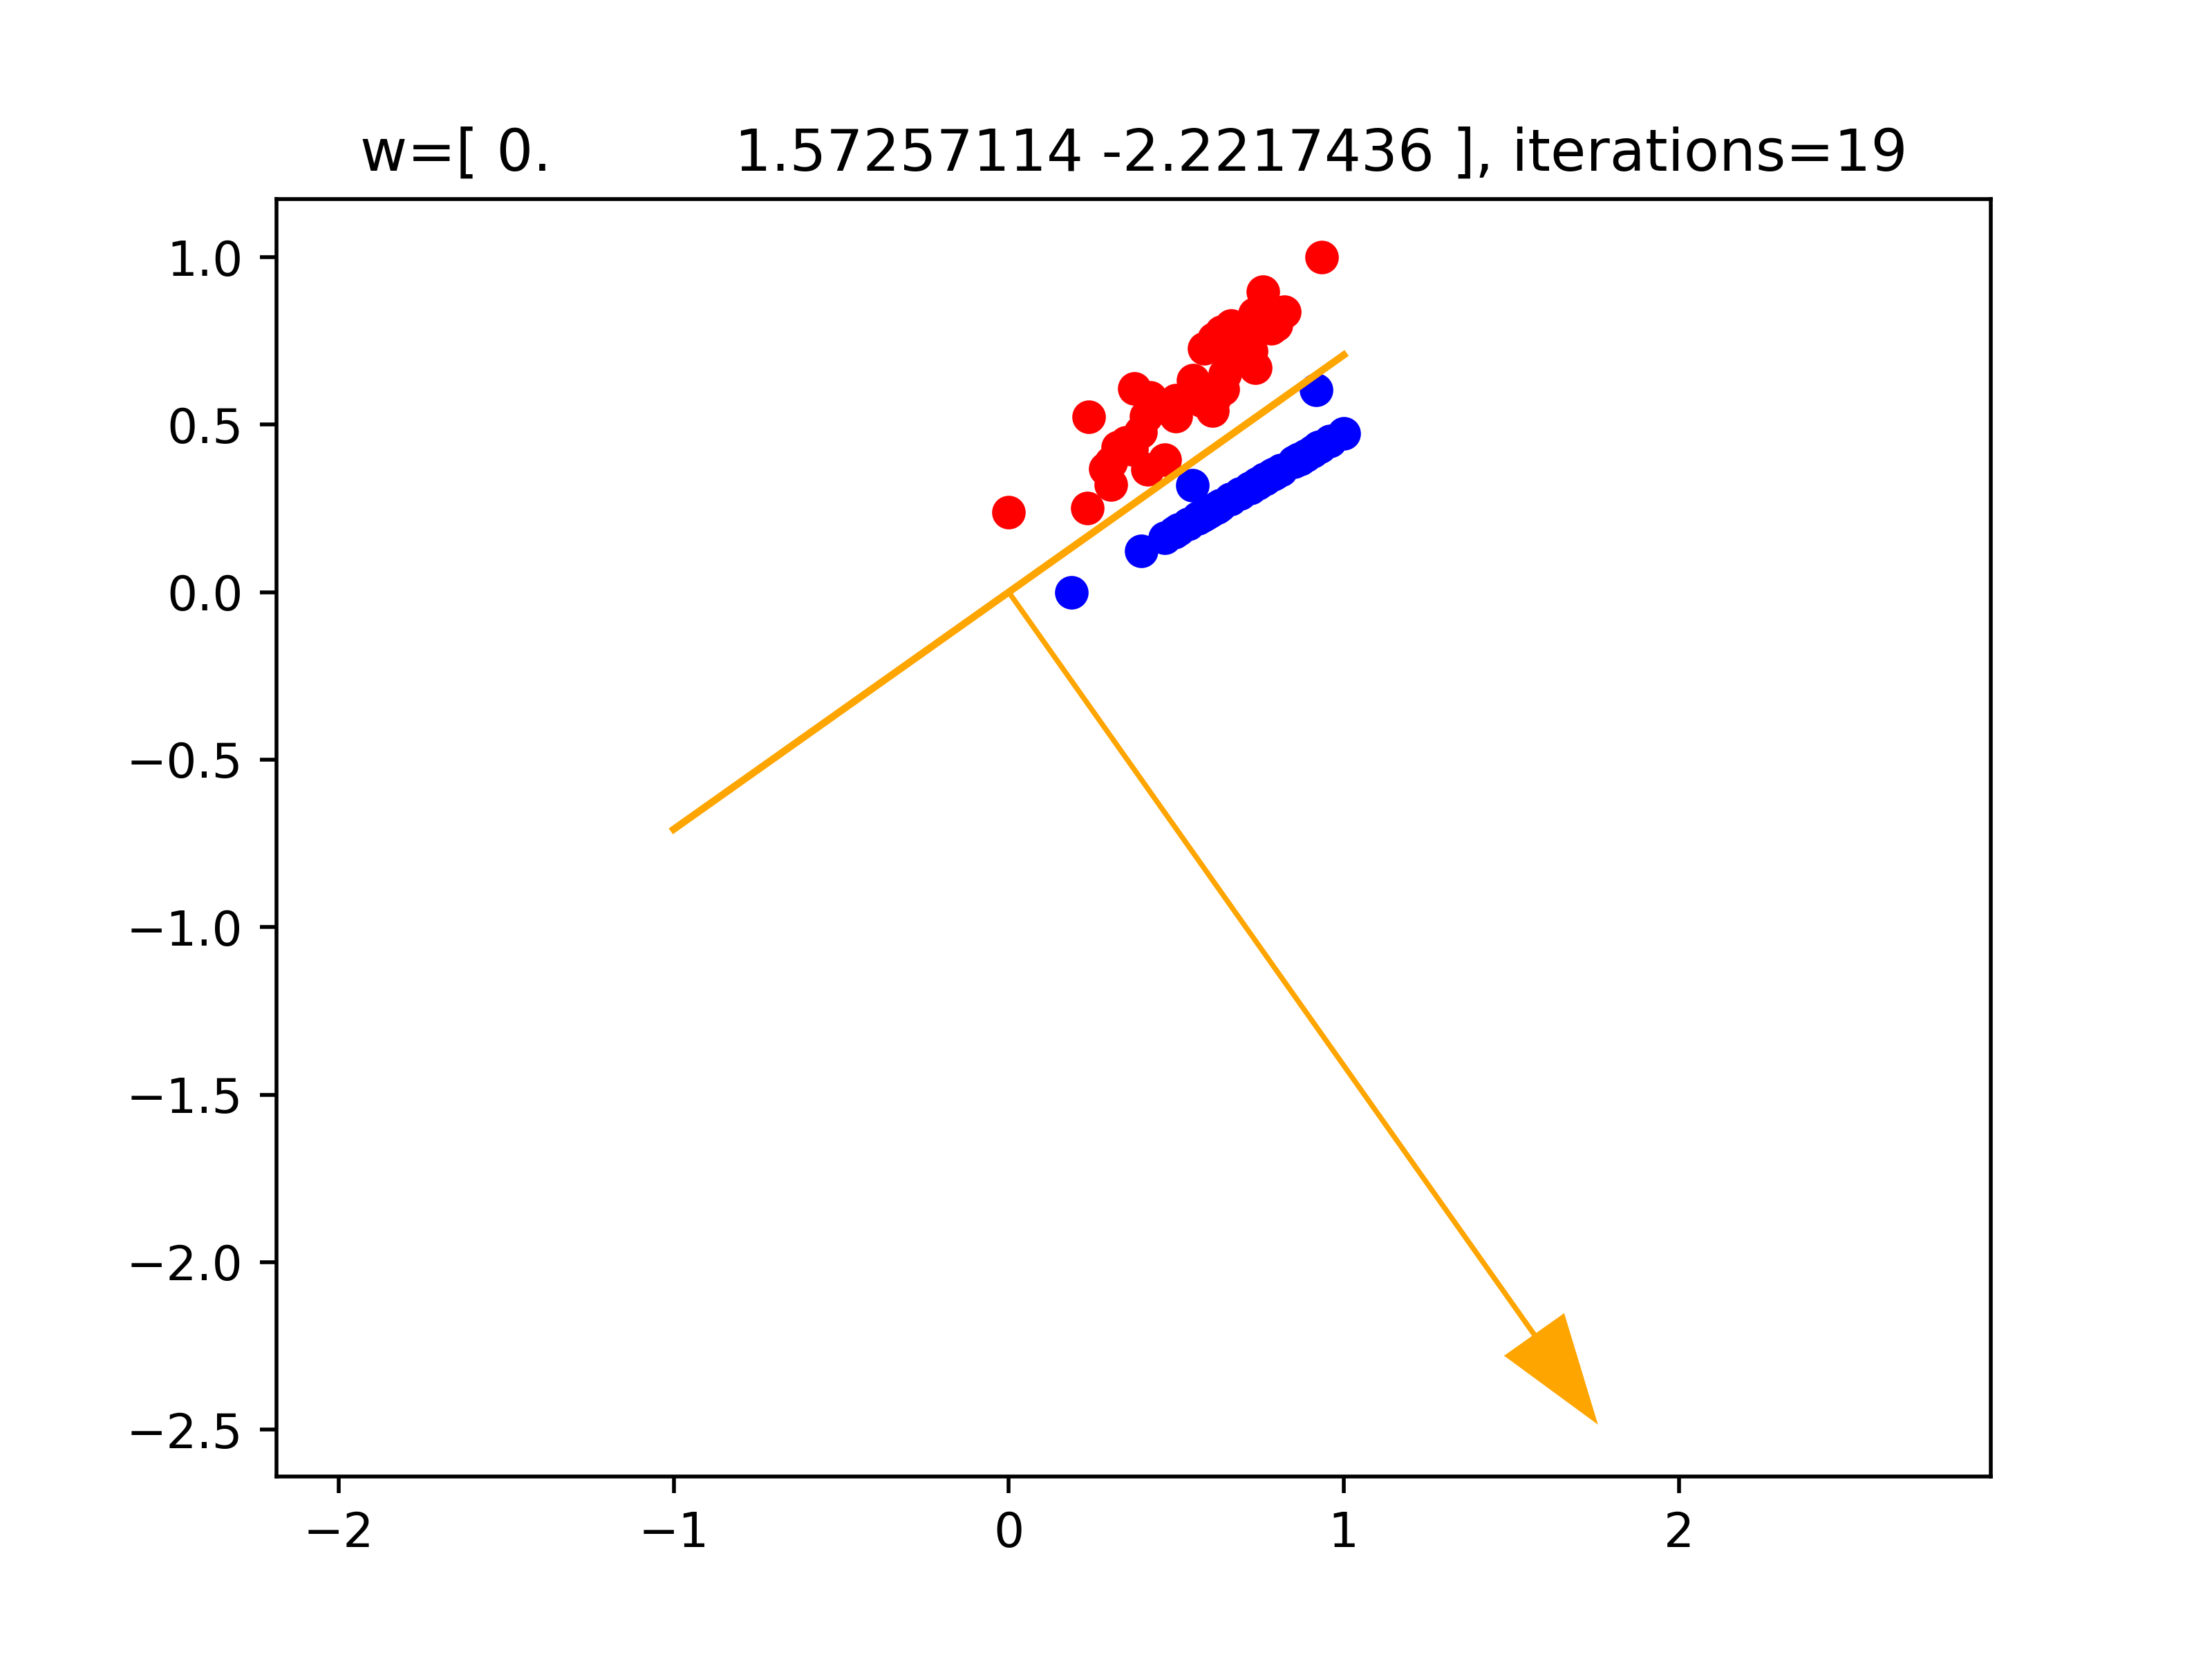
\includegraphics[scale=0.7]{Q3b.png}

Code screenshot: 

\includegraphics[scale=0.5]{code:Q3b.png}

\newpage
\subsection*{c}

Pseudo code to implement \emph{Positive Winnow} algorithm:

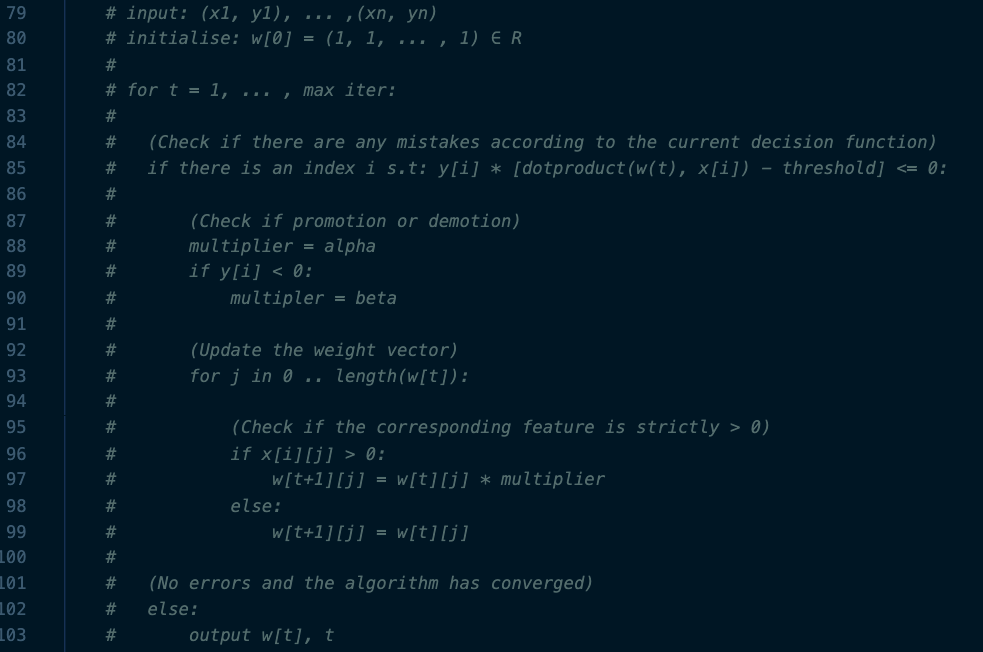
\includegraphics[scale=0.43]{psuedo:code:q3c.png}

Note that I am using \(t\) as the \(w\) vector iteration number and \(i\) as the observation that the mistake
occurred at. This is the other way around in the provided paper.

\includegraphics[scale=0.9]{q3c.png}

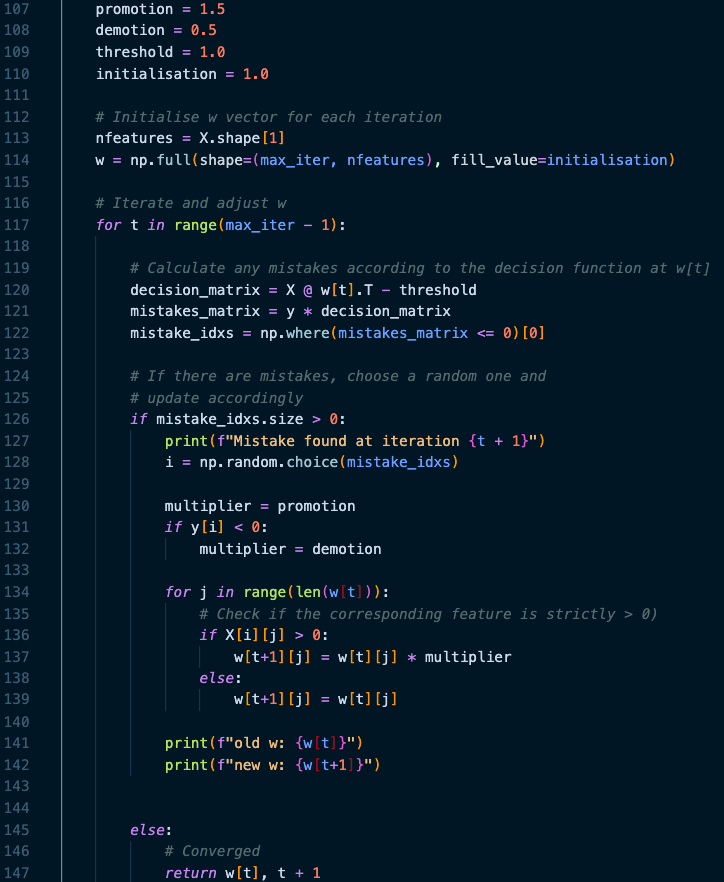
\includegraphics[scale=0.5]{code:q3c.png}

\newpage
\subsection*{d}

\includegraphics[scale=0.4]{psuedo:code:q3d.png}

\includegraphics[scale=0.9]{q3d.png}

\includegraphics[scale=0.4]{code:q3d.png}

\subsection*{e}

\includegraphics[scale=0.4]{psuedo:code:q3e.png}

\includegraphics[scale=0.9]{q3e.png}

\includegraphics[scale=0.4]{code:q3e.png}

The balanced and modified Winnow algorithms have 2 main differences. The first is
how the algorithms consider a mistake. The Balanced Winnow will consider an incoming 
data point mistake if the decision function predicts it incorrectly 
(\(y[t] * sign(\langle x_{t}, u_{i} \rangle - \langle x_{t}, v_{i} \rangle - \theta_{th}) \leq 0\)).
The Modified Winnow considers a data point a mistake if the decision function predicts
the incoming data point \emph{within a margin}. 
(\(y[t] * sign(\langle x_{t}, u_{i} \rangle - \langle x_{t}, v_{i} \rangle - \theta_{th}) \leq M\))
The second is how the vectors update when a mistake occurs. In the Modified Winnow, the multiplicative correction 
depends on the particular feature weight of the incoming example (\(x_{t}^{j}\)), rather than 
correcting by a constant (\(\alpha\) or \(\beta\)). This makes the corrections
in the Modified Winnow more aggressive.

\end{document}
